% !TEX root = ../OT4ML.tex

\chapter{Generative Models via Transportation}
\index{generative model}% strictindex
\label{sec-generative-models-transportation}

To construct generative models, we now prescribe measure evolutions that need not be gradient flows of a fixed energy. This gives additional freedom to choose paths that are easy to learn and sample. We study flow matching and diffusion, one-step generators, moment measures, token evolution and Gaussian models.

The sampling task is to transport a simple reference law $\alpha=\alpha_0$ (typically Gaussian) to a data law $\beta=\alpha_1$. For a nonatomic reference on a standard Borel space, a measurable map $T$ with $T_\sharp\alpha=\beta$ exists, but this does not supply a tractable sampler. Instead, a well-posed velocity field and continuity equation as in Section~\ref{sec-measure-evolutions} give $(T_t)_\sharp\alpha_0=\alpha_t$; when the flow reaches the endpoint, $X_1=T_1(X_0)$ samples $\beta$ from $X_0\sim\alpha$. The endpoint and numerical qualifications are detailed in~\eqref{eq-flow-matching-sampling-map} below. For a general transport perspective on diffusion models, see~\cite{Peyre2026OptimalDiffusionTransports}.
\index{Wasserstein!gradient}% strictindex
\index{gradient!flow}% strictindex
\index{Wasserstein!gradient flow}% strictindex
\index{token measure}% strictindex
\index{one-step generative model}% strictindex

\section{Generative Models via Flow Matching}
\label{sec-generative-flow-matching}
\index{flow matching}% strictindex
\index{generative model}% strictindex

Flow matching constructs a generative map by learning an Eulerian velocity field for a prescribed interpolation. The key computational insight is that an unconstrained regression produces one field satisfying the continuity equation. It need not be the minimum-kinetic-energy Wasserstein tangent of that same measure curve.
\index{velocity field}% strictindex
\index{continuity equation}% strictindex

After constructing an interpolation $\alpha_t$, the weighted-Poisson problem~\eqref{eq:least-square-field-explicit}, whenever its finite-action assumptions hold, selects its minimum-\(L^2(\alpha_t)\)-norm tangent in the closure of gradient fields. A parametric push-forward provides another admissible field directly: the conditional expectation of the latent path velocities. It is learned by an unconstrained least-squares regression and therefore avoids a Poisson solve. The two representatives differ in general by a field \(w_t\) satisfying \(\diverg(\alpha_t w_t)=0\); they coincide when the conditional-expectation field is itself in the closed Wasserstein tangent-gradient space, as in the Gaussian-endpoint example below.
\index{conditional!expectation}% strictindex
\index{push-forward}% strictindex

\paragraph{Deterministic interpolants.}
\index{deterministic interpolant}% strictindex
\index{temporal noise}% strictindex
\index{stochastic!interpolant}% strictindex

An interpolant specifies sample paths whose positions and velocities are easy to evaluate. Sampling these pairs turns the reconstruction of an Eulerian field into regression (Proposition~\ref{prop-flow-matching-vector-field}). The pathwise velocity need not equal the Eulerian velocity when paths cross: regression averages velocities at the current position.
\begin{defn}[Deterministic interpolant]\label{def-deterministic-interpolant}
Let $\pi\in\Pp(\RR^{d'})$ be a latent law. A deterministic interpolant between $\alpha_0$ and $\alpha_1$ is a jointly measurable family $I_t:\RR^{d'}\to\RR^d$ such that $t\mapsto I_t(u)$ is absolutely continuous for $\pi$-almost every $u$, its derivative is jointly measurable, and $\int_0^1\int\norm{\partial_tI_t(u)}\d\pi(u)\d t<\infty$. It satisfies $(I_0)_\sharp\pi=\alpha_0$, $(I_1)_\sharp\pi=\alpha_1$ and induces
\begin{equation}\label{eq:interp-coupling}
 \alpha_t=(I_t)_\sharp\pi,\qquad t\in[0,1].
\end{equation}
\end{defn}
Once the latent sample is fixed, its path has no further temporal randomness. An endpoint coupling is the basic choice of latent law; extra static randomness can be included in the same definition by enlarging the latent variable.

\begin{example}[Linear two-endpoint deterministic interpolants]
	Set $d'=2d$, write $(x,y)\in\RR^d\times\RR^d$, and choose the straight path $I_t(x,y)=(1-t)x+ty$. If $\pi$ has marginals $(\alpha_0,\alpha_1)$, then $\alpha_t=(I_t)_\sharp\pi$ interpolates between the two endpoint laws. For independent endpoints only, $\pi=\alpha_0\otimes\alpha_1$, this is the rescaled convolution $\alpha_t=(D_{1-t})_\sharp\alpha_0*(D_t)_\sharp\alpha_1$, where $D_s(x)=sx$; see Definition~\ref{def-measure-convolution}. This identity does not hold for a general dependent coupling.
	With this linear path and an arbitrary coupling $\pi$, the regression below is the common core of flow matching and rectified flow: Lipman et al.\ emphasize conditional probability paths and simulation-free training of continuous normalizing flows, while rectified flow emphasizes straight couplings, reflow, and the possibility of reducing transport costs and discretization error~\cite{Lipman2022FlowMatching,Liu2023RectifiedFlow}.
\index{flow!rectified}% strictindex
\index{flow matching}% strictindex

	More complex constructions are possible when sampling from $\pi$ remains simple. Static auxiliary randomness is still handled by enlarging the latent variable, while Brownian noise leads to the diffusion correction described below; this is the broader stochastic-interpolant viewpoint connecting deterministic flows, probability-flow ODEs and diffusion SDEs~\cite{Albergo2025StochasticInterpolants}.
\index{flow!probability ODE}% strictindex
\end{example}
\index{flow!continuous normalizing}% strictindex
\index{reflow}% strictindex
\index{discretization error}% strictindex
\index{latent!variable}% strictindex
\index{conditional!probability}% strictindex
\index{flow!normalizing}% strictindex
\index{probability path}% strictindex
\index{flow matching}% strictindex
\index{flow!rectified}% strictindex
\index{flow!probability ODE}% strictindex
\index{trivial coupling}% strictindex

\begin{rem}[Independent and optimal-transport couplings]
The two most common constructions use either independent endpoint samples or an optimal-transport coupling. For $\pi=\alpha_0\otimes\alpha_1$, if $\alpha_0=n^{-1}\sum_i\delta_{x_i}$ and $\alpha_1=m^{-1}\sum_j\delta_{y_j}$, then $\alpha_t=(nm)^{-1}\sum_{i,j}\delta_{I_t(x_i,y_j)}$ has at most $nm$ atoms, since some locations can coincide. At the opposite geometric extreme, if $T$ is the quadratic-optimal Brenier map from $\alpha_0$ to $\alpha_1$, the coupling $\pi=(\Id,T)_\sharp\alpha_0$ with the straight interpolant gives $\alpha_t=((1-t)\Id+tT)_\sharp\alpha_0$, namely the McCann displacement interpolation. Figure~\ref{fig:generative-flow-matching-interpolants} separates these two choices of endpoint coupling from the separate choice of path joining each pair.
\index{Dirac mass}% strictindex
\end{rem}

\begin{figure}[H]
\centering
\begin{tabular}{@{}ccc@{}}
\small product pairing & \small OT pairing & \small curved bridge \\[-.15em]
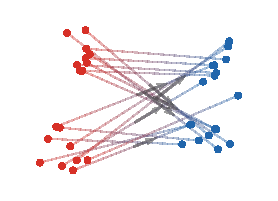
\includegraphics[width=.30\linewidth]{figures/generative-flow-matching-interpolants/product-linear.pdf} &
\index{flow matching}% strictindex
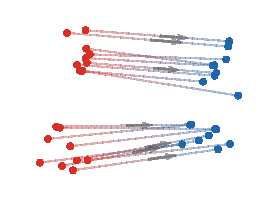
\includegraphics[width=.30\linewidth]{figures/generative-flow-matching-interpolants/ot-linear.pdf} &
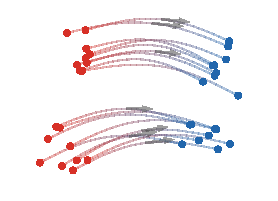
\includegraphics[width=.30\linewidth]{figures/generative-flow-matching-interpolants/curved-bridge.pdf}
\end{tabular}
\caption{\emph{Flow matching interpolants between the same empirical source and target measures.} A product-style random pairing produces crossing paths, an OT pairing gives direct displacement rays, and a curved bridge changes the path geometry while keeping the same endpoints. Gray arrows mark representative midpoint velocities $\partial_t I_t$.}
\label{fig:generative-flow-matching-interpolants}
\end{figure}

\paragraph{Learning a flow field.}
\index{flow matching}% strictindex

This interpolation is not directly useful for sampling from $\beta$, but it can be used to define a flow field $v_t$ so that the Eulerian advection equation~\eqref{eq:eulerian-advection} holds.
%
This flow field is computed by an unconstrained least-squares problem: it averages the path velocities conditional on the current position. The conditional-law interpretation uses disintegration, as in Definition~\ref{def-conditional-ot}, rather than selecting a single latent sample for each position.
\index{conditional!expectation}% strictindex

\begin{prop}[Flow matching vector field]\label{prop-flow-matching-vector-field}
	Assume that $t\mapsto I_t(u)$ is absolutely continuous for $\pi$-almost every $u$, that its derivative $(t,u)\mapsto\partial_t I_t(u)$ is jointly measurable, and that \(\int_0^1\!\int_{\RR^{d'}}\norm{\partial_t I_t(u)}^2\d\pi(u)\d t<+\infty\).
	Let \(U\sim\pi\) and \(X_t=I_t(U)\), so that \(X_t\sim\alpha_t\).
	For almost every $t$, consider the flow-matching problem over \(v_t\in L^2(\alpha_t;\RR^d)\)
\index{flow matching}% strictindex
	\begin{equation}
		\min_{v_t} \int_{\RR^{d'}} \norm{v_t(I_t(u)) - [\partial_t I_t](u)}^2 \, \d\pi(u). \label{eq:flow-matching}
	\end{equation}
	Its minimizer is characterized $\alpha_t$-almost everywhere by
\index{conditional!expectation}% strictindex
	\begin{equation}\label{eq:flow-match-conditional}
		v_t(x)=\EE\bigl[\partial_t I_t(U)\mid X_t=x\bigr].
	\end{equation}
	There is a jointly measurable choice \((t,x)\mapsto v_t(x)\), obtained by disintegrating \(\d t\,\pi(\d u)\) under \((t,u)\mapsto(t,I_t(u))\). For this choice, $v_t\in L^2(\alpha_t;\RR^d)$ for almost every $t$, and the pair $(\alpha_t,v_t)$ satisfies the continuity equation~\eqref{eq:eulerian-advection} in the distributional sense on $(0,1)\times\RR^d$.
\index{continuity equation}% strictindex
\end{prop}

\begin{proof}
	The push-forward identity reads \(\int_{\RR^d}\varphi(x)\,\d\alpha_t(x)=\int_{\RR^{d'}}\varphi(I_t(u))\,\d\pi(u)\) for every bounded continuous test function $\varphi$.
\index{push-forward}% strictindex
	For almost every $t$, the minimizer in~\eqref{eq:flow-matching} is the orthogonal projection in $L^2(\pi;\RR^d)$ of the latent velocity $\partial_t I_t(u)$ onto the closed subspace of functions that depend on $u$ only through $I_t(u)$. This projection is the conditional expectation~\eqref{eq:flow-match-conditional}. Equivalently, disintegration of the joint measure \(\d t\,\pi(\d u)\) by the map \((t,u)\mapsto(t,I_t(u))\) supplies a jointly measurable version. Conditional Jensen gives \(\int\norm{v_t}^2\d\alpha_t\leq\int\norm{\partial_t I_t}^2\d\pi\),
	so the Eulerian velocity is square-integrable in space--time. Its defining conditional-expectation identity is, for every \(m\in L^2(\alpha_t;\RR^d)\),
\index{conditional!expectation}% strictindex
\index{flow matching}% strictindex
	\begin{equation}\label{eq:v_t}
		\int \dotp{m(x)}{v_t(x)} \, \d\alpha_t(x)
		=
		\int \dotp{m(I_t(u))}{[\partial_t I_t](u)} \, \d\pi(u).
	\end{equation}

	We now prove that this field transports the curve $(\alpha_t)_t$. Testing first with \(\varphi\in C_c^\infty(\RR^d)\), and then integrating against compactly supported smooth functions of time, gives the distributional formulation on space--time. The fixed-time weak identity for
	$\partial_t\alpha_t+\diverg(\alpha_t v_t)=0$ is that, for every $\varphi\in C_c^\infty(\RR^d)$,
	\begin{equation}\label{eq:flow-matching-weak-target}
		\frac{\d}{\d t}\int\varphi(x)\,\d\alpha_t(x)
		-
		\int\dotp{v_t(x)}{\nabla\varphi(x)}\,\d\alpha_t(x)
		=0.
	\end{equation}
	By the pathwise chain rule, $t\mapsto\varphi(I_t(u))$ is absolutely continuous for $\pi$-almost every $u$. The space--time integrability assumption and Fubini's theorem justify integration of its derivative, so the push-forward identity gives, for almost every $t$,
\index{push-forward}% strictindex
\index{flow matching}% strictindex
	\begin{equation}\label{eq:flow-matching-test-derivative}
		\frac{\d}{\d t}\int \varphi(x)\d\alpha_t(x)
		=
		\int \dotp{\nabla\varphi(I_t(u))}{[\partial_t I_t](u)}\d\pi(u).
	\end{equation}
	On the other hand, applying~\eqref{eq:v_t} with $m=\nabla\varphi$ gives
	\begin{equation}\label{eq:flow-matching-velocity-test}
		\int\dotp{v_t(x)}{\nabla\varphi(x)}\,\d\alpha_t(x)
		=
		\int \dotp{\nabla\varphi(I_t(u))}{[\partial_t I_t](u)}\d\pi(u).
	\end{equation}
	Comparing~\eqref{eq:flow-matching-test-derivative} and~\eqref{eq:flow-matching-velocity-test} yields~\eqref{eq:flow-matching-weak-target}, which is the desired continuity equation.
\index{continuity equation}% strictindex
\index{flow matching}% strictindex
\end{proof}

\index{conditional!expectation}% strictindex
\index{disintegration}% strictindex
%
Numerically, $(x,t) \mapsto v_t(x)$ can be parameterized by a neural network, for example a U-Net for image data~\cite{RonnebergerFischerBrox2015UNet}. The least-squares regression~\eqref{eq:flow-matching} can then be optimized over the network parameters using stochastic optimization algorithms.
\index{stochastic!gradient}% strictindex
\index{flow matching}% strictindex
%

\paragraph{Sampling algorithm.}
Once the field $v_t$ has been estimated by the tractable regression~\eqref{eq:flow-matching}, generation amounts to integrating its characteristics. For a sufficiently regular version of the exact population field, let $T_t$ denote the flow map solving
\begin{equation}\label{eq-flow-matching-sampling-map}
	\partial_tT_t(x)=v_t(T_t(x)),
	\qquad T_0(x)=x.
\end{equation}
Assume that this ODE generates a unique measurable flow on every compact subinterval of $[0,1)$ and that the continuity equation is unique in the corresponding solution class. Since the exact field transports the prescribed curve, $(T_t)_\sharp\alpha_0=\alpha_t$ for $t<1$. If the flow map extends to $t=1$, then $(T_1)_\sharp\alpha_0=\alpha_1$; consequently, $X_0\sim\alpha_0$ implies $T_1(X_0)\sim\alpha_1$. Numerically, one draws independent samples from the simple reference law $\alpha_0$ and approximates $T_1$ by solving~\eqref{eq-flow-matching-sampling-map} with the regressed field, so the resulting endpoint law is only approximately $\alpha_1$. For singular endpoints, even the exact flow may instead satisfy only $(T_t)_\sharp\alpha_0=\alpha_t\rightharpoonup\alpha_1$ as $t\uparrow1$, while the velocity or its spatial derivative becomes singular.
\index{transport!map}% strictindex
\index{continuity equation}% strictindex

This inference stage can be expensive because every generated sample requires many neural-field evaluations along an ODE trajectory. Section~\ref{sec-one-step-generative-models} presents the opposite tradeoff: repeated flow estimation or distillation makes training more expensive, but the final sampler is a single network evaluation.

\paragraph{Connection with diffusion models.}\label{par-diffusion-model-connection}
\index{diffusion model}% strictindex

Diffusion models build on score matching~\cite{Hyvarinen2005ScoreMatching}, denoising score matching~\cite{Vincent2011DenoisingScoreMatching}, noising chains~\cite{SohlDickstein2015DeepUnsupervised,Ho2020DDPM}, and score-based generative modeling~\cite{Song2019ScoreMatchingGenerative,Song2021ScoreSDE}. With an independent isotropic Gaussian endpoint, the convolution construction above produces their smoothed marginal paths; the associated probability-flow ODE is trained through a score or velocity regression.

For this paragraph we follow the \emph{forward noising} direction: $X_0\sim\beta$ is data, $Z\sim\alpha=\Gaussian(0,\Id)$ is independent noise, and $\beta_t=\operatorname{Law}((1-t)X_0+tZ)$ runs from data to noise. Thus the corresponding generative path is the time reversal $\alpha_t=\beta_{1-t}$. Apply~\eqref{eq:flow-matching} to this noising interpolant and reverse the resulting ODE for sampling. Tweedie's identity gives its explicit gradient velocity.

Figure~\ref{fig:generative-diffusion-2d-forward-backward} illustrates at this point how the scalar coefficients of the interpolant separately control contraction of the data centers and growth of the Gaussian noise.

\begin{figure}[ht]
\centering
\begin{tabular}{@{}c@{}}
\small linear bridge, $a_t=1-t$, $b_t=t$ \\[-.15em]
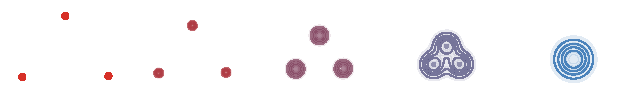
\includegraphics[width=.72\linewidth]{figures/generative-diffusion-2d-forward-backward/forward-density-linear.pdf} \\[.15em]
\small OU/variance-preserving bridge, $a_t=\cos(\pi t/2)$, $b_t=\sin(\pi t/2)$ \\[-.15em]
\index{bridge!OU}% strictindex
\index{bridge!variance-preserving}% strictindex
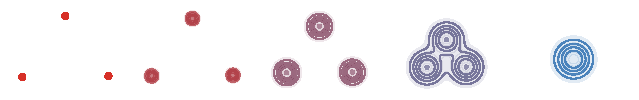
\includegraphics[width=.72\linewidth]{figures/generative-diffusion-2d-forward-backward/forward-density-ou.pdf}
\end{tabular}
\caption{\emph{Two-dimensional noising paths from three Dirac masses to a single Gaussian.} The top row shows the linear interpolation $X_t=(1-t)X_0+tZ$, whose component centers move linearly toward the origin and whose covariance grows like $(t\sigma)^2\Id$. The bottom row uses the variance-preserving Ornstein--Uhlenbeck coefficients $a_\tau=e^{-\tau}$ and $b_\tau=\sqrt{1-e^{-2\tau}}$, reparametrized by $\tau=-\log\cos(\pi t/2)$ so that $a_t=\cos(\pi t/2)$ and $b_t=\sin(\pi t/2)$. It has the same endpoints but a different speed of contraction and noising.}
\index{Ornstein-Uhlenbeck@Ornstein--Uhlenbeck!process}% strictindex
\label{fig:generative-diffusion-2d-forward-backward}
\end{figure}
%
In this setting, $v_t$ is also the solution of the constrained least-squares problem~\eqref{eq:least-square-field-explicit}. The regression~\eqref{eq:flow-matching} is computationally simpler because the continuity equation has already been enforced by the chosen interpolant.
\index{continuity equation}% strictindex
%
To prove this, we rely on Tweedie's formula~\cite{Efron2011Tweedie}, which expresses the optimal Gaussian denoiser through the score, i.e.\ the gradient of the log-density.
\index{Gaussian!denoiser}% strictindex
\index{score function}% strictindex
\index{Tweedie identity}% strictindex

\begin{proposition}[Tweedie identity]\label{prop:Tweedie}
Let $W$ be a random vector in $\RR^{d}$ with law $\beta\in\Pp_1(\RR^d)$.
For $\sigma>0$, let $Z\sim\Gaussian(0,\Id)$ be independent of $W$ and observe
\[
Y=W+\sigma Z.
\]
Denote by $\rho_\sigma$ the smooth positive density of \(\beta_\sigma=\beta * \Gaussian(0,\sigma^{2}\Id)\), which is the law of $Y$.
Then the conditional mean admits the following everywhere-defined version:
\[
\EE\bigl[W\mid Y=y\bigr]
      =y+\sigma^{2}\nabla \log \rho_\sigma(y)
\qquad\text{for all } y \in \RR^{d}.
\]
\end{proposition}

\begin{proof}
Let $\varphi_\sigma$ be the $\Gaussian(0,\sigma^{2}\Id)$ density. Bayes' rule gives \(\EE[W\mid Y=y]=\rho_\sigma(y)^{-1}\int_{\RR^{d}} w\varphi_\sigma(y-w)\,\d\beta(w)\).
Differentiating the Gaussian convolution under the integral sign and using
$
\nabla_y\varphi_\sigma(y-w)
     = -\sigma^{-2}(y-w)\,\varphi_\sigma(y-w)
$
yields
\[
\nabla\rho_\sigma(y)
= \int \nabla_y\varphi_\sigma(y-w)\,\d\beta(w)
= -\sigma^{-2}\Bigl(y-\EE[W\mid Y=y]\Bigr)\,\rho_\sigma(y).
\]
Rearranging finishes the proof.
\end{proof}


Tweedie's identity now turns the conditional expectation defining flow matching into an explicit score field for a Gaussian endpoint.

\begin{proposition}[Gaussian-endpoint flow-matching field]\label{prop:flow}
\index{flow matching}% strictindex
Let \(\beta\in\Pp_2(\RR^d)\), let $X_0\sim\beta$, and let $Z\sim\Gaussian(0,\Id)$ be independent.
For $t\in(0,1)$ set \(X_t=(1-t)X_0+tZ\) and \(\beta_t=\operatorname{Law}(X_t)=\rho_t\,\d x\). The minimizer $v^\star:\RR^d\times(0,1)\to\RR^d$ of the flow-matching regression~\eqref{eq:flow-matching} is
\[
v^\star(x,t)
= -\frac{1}{1-t}\,x \;-\; \frac{t}{1-t}\,\nabla\log\rho_t(x)
\qquad (x\in\RR^{d},\;t\in(0,1)).
\]
In particular, for each $t\in(0,1)$ this field is the gradient field \(v^\star(\cdot,t)=-\nabla\bigl(\norm{\cdot}^2/[2(1-t)]+t\log\rho_t/(1-t)\bigr)\).
\end{proposition}

\begin{proof}
Fix $t\in(0,1)$ and write $W=(1-t)X_0$ and $\sigma=t$, so that
$X_t=W+\sigma Z$ matches the setting of Proposition~\ref{prop:Tweedie}.
\index{Tweedie identity}% strictindex
Conditional expectations satisfy
\index{conditional!expectation}% strictindex
$
v^\star(x,t)
= \EE[Z-X_0\mid X_t=x]
= \frac{1}{t}\,\EE[X_t-W\mid X_t=x]
  -\,\frac{1}{1-t}\,\EE[W\mid X_t=x].
$
Applying Proposition~\ref{prop:Tweedie} to $\EE[W\mid X_t=x]$ and
\index{Tweedie identity}% strictindex
noting $\EE[Z\mid X_t=x]=-t\nabla\log\rho_t(x)$
gives the claimed formula.
\end{proof}

Figure~\ref{fig:generative-diffusion-1d-forward-backward} shows both directions of this construction: the prescribed interpolation noising the data and the same probability-flow ODE integrated backward for sampling.

\begin{figure}[ht]
\centering
\begin{tabular}{@{}cc@{}}
\small forward noising & \small reverse probability flow \\[-.15em]
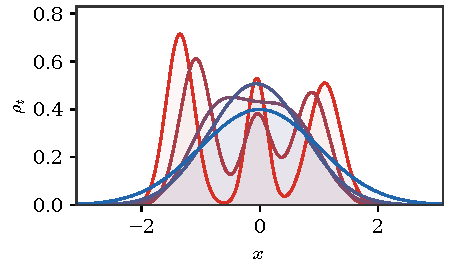
\includegraphics[width=.43\linewidth]{figures/generative-diffusion-1d-forward-backward/forward-densities.pdf} &
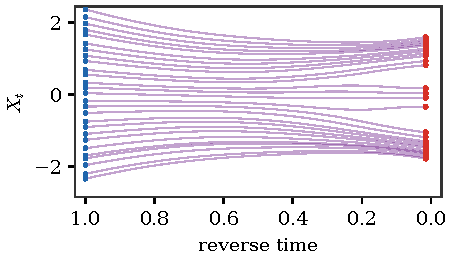
\includegraphics[width=.43\linewidth]{figures/generative-diffusion-1d-forward-backward/backward-trajectories.pdf}
\end{tabular}
\caption{\emph{One-dimensional diffusion bridge for a Gaussian-mixture data law.} The forward path $X_t=(1-t)X_0+tZ$ smooths the red data density toward a blue Gaussian endpoint. Reversing the probability-flow ODE transports stratified, slightly jittered seeds representing that endpoint back toward the data modes, making the splitting of trajectories across mixture components visible.}
\index{Gaussian!mixture}% strictindex
\index{flow!probability ODE}% strictindex
\label{fig:generative-diffusion-1d-forward-backward}
\end{figure}

The same probability-flow intuition is explicit in two dimensions. For a discrete data law, or more generally for a Gaussian mixture, the noising density is a Gaussian mixture whose score can be evaluated in closed form. If $\beta=\sum_jw_j\Gaussian(c_j,\Sigma_j)$ and the independent noise is $Z\sim\Gaussian(0,\sigma^2\Id)$, the schedule $X_t=a_tX_0+b_tZ$ has component means $a_tc_j$ and covariances $a_t^2\Sigma_j+b_t^2\sigma^2\Id$. In particular, for discrete data ($\Sigma_j=0$) and the linear bridge, $\beta_t=\sum_jw_j\Gaussian((1-t)c_j,(t\sigma)^2\Id)$. If $\rho_t$ denotes its density and $s_t=\nabla\log\rho_t$ its score, the scaled version of Proposition~\ref{prop:flow} gives $v_t(x)=-(x+t\sigma^2s_t(x))/(1-t)$.
\index{noising schedule}% strictindex
\index{score function}% strictindex

\paragraph{When is the induced map optimal?}

Integrating the learned velocity gives a deterministic map from $\alpha_0$ to $\alpha_1$, but this map is not automatically the Brenier optimal map. It is optimal only in special cases where the accumulated flow remains the gradient of a convex potential. The Gaussian product-coupling case already shows the precise obstruction: the interpolated covariances are simple, the velocity is affine, but the terminal map can contain a hidden rotational part. This phenomenon, and its extensions to rectified flows and mixtures, is analyzed in depth in~\cite{HertrichChambolleDelon2025RectifiedOT}.
\index{convex!potential}% strictindex
\index{product!coupling}% strictindex
\index{flow!rectified}% strictindex
Quadratic optimal transport between Gaussian measures is developed in Section~\ref{sec-gaussian-bures}; in particular, Proposition~\ref{prop-gaussian-w2-bures} and~\eqref{eq-bures-map} prove the formula for $T^{\rm OT}$ used below.

\begin{prop}[Gaussian flow matching and optimality]\label{prop-gaussian-flow-matching-optimality}
\index{Gaussian!flow matching}% strictindex
	Let $\Sigma_0,\Sigma_1\succ0$ and let $X_0\sim\Gaussian(0,\Sigma_0)$ and $X_1\sim\Gaussian(0,\Sigma_1)$ be independent. Consider the linear flow-matching interpolation
\index{flow matching}% strictindex
	\[
		X_t=(1-t)X_0+tX_1,
		\qquad
		\alpha_t=\operatorname{Law}(X_t)=\Gaussian(0,\Sigma_t),
	\]
	where $\Sigma_t=(1-t)^2\Sigma_0+t^2\Sigma_1$. Then the exact flow-matching velocity is affine, $v_t(x)=A_tx$, with $A_t=\bigl(t\Sigma_1-(1-t)\Sigma_0\bigr)\Sigma_t^{-1}$.
\index{flow matching}% strictindex
	The induced flow map $T_t^{\rm FM}$ from $\alpha_0$ to $\alpha_t$ is
\index{flow!map}% strictindex
	\begin{equation}\label{eq-gaussian-product-fm-map}
		T_t^{\rm FM}
		=
		\Sigma_0^{1/2}
		\Bigl((1-t)^2\Id+t^2\Sigma_0^{-1/2}\Sigma_1\Sigma_0^{-1/2}\Bigr)^{1/2}
		\Sigma_0^{-1/2}.
	\end{equation}
	\eqllead{In particular,}{eq-gaussian-product-fm-terminal-map}{
		T_1^{\rm FM}
		=
		\Sigma_0^{1/2}
		\bigl(\Sigma_0^{-1/2}\Sigma_1\Sigma_0^{-1/2}\bigr)^{1/2}
		\Sigma_0^{-1/2}.
	}
	This terminal map coincides with the quadratic optimal transport map
\index{transport!map}% strictindex
	\begin{equation}\label{eq-gaussian-brenier-map-comparison}
		T^{\rm OT}
		=
		\Sigma_0^{-1/2}
		\bigl(\Sigma_0^{1/2}\Sigma_1\Sigma_0^{1/2}\bigr)^{1/2}
		\Sigma_0^{-1/2}
	\end{equation}
	if and only if $\Sigma_0\Sigma_1=\Sigma_1\Sigma_0$.
\end{prop}

\begin{proof}
	The conditional-expectation formula gives
\index{conditional!expectation}% strictindex
	\(v_t(x)=\EE[X_1-X_0\mid X_t=x]\).
	Since all variables are jointly Gaussian, this conditional expectation is linear and
	\[
		v_t(x)
		=
		\operatorname{Cov}(X_1-X_0,X_t)\operatorname{Cov}(X_t)^{-1}x
		=
		\bigl(t\Sigma_1-(1-t)\Sigma_0\bigr)\Sigma_t^{-1}x,
	\]
		which proves the stated velocity formula. To solve the characteristic equation, whiten the source by setting \(C=\Sigma_0^{-1/2}\Sigma_1\Sigma_0^{-1/2}\) and \(\widetilde X_t=\Sigma_0^{-1/2}X_t\).
	In these coordinates the source covariance is $\Id$ and
	\(\widetilde\Sigma_t=(1-t)^2\Id+t^2C\).
	Because $\Id$ and $C$ commute, the affine flow map in whitened coordinates is simply $\widetilde T_t=\widetilde\Sigma_t^{1/2}$. Indeed,
\index{flow!map}% strictindex
	$\frac{\d}{\d t}\widetilde\Sigma_t^{1/2}=\bigl(tC-(1-t)\Id\bigr)\widetilde\Sigma_t^{-1/2}$, which is exactly the equation $\dot{\widetilde T}_t=\widetilde A_t\widetilde T_t$ with $\widetilde T_0=\Id$. Returning to the original coordinates gives~\eqref{eq-gaussian-product-fm-map}, and $t=1$ gives~\eqref{eq-gaussian-product-fm-terminal-map}.

		Both $T_1^{\rm FM}$ and $T^{\rm OT}$ push $\Gaussian(0,\Sigma_0)$ to $\Gaussian(0,\Sigma_1)$. The Brenier map between nondegenerate Gaussians is the unique symmetric positive definite linear map with this property. Hence $T_1^{\rm FM}=T^{\rm OT}$ if and only if $T_1^{\rm FM}$ is symmetric positive definite. The map $T_1^{\rm FM}$ is similar to $C^{1/2}$, so if it is symmetric then it is automatically positive definite. It remains to characterize symmetry. Since $C^{1/2}$ is symmetric positive definite, \((T_1^{\rm FM})^\top=\Sigma_0^{-1/2}C^{1/2}\Sigma_0^{1/2}\).
\index{Brenier!map}% strictindex
	Thus symmetry of $T_1^{\rm FM}$ is equivalent to
	$\Sigma_0 C^{1/2}=C^{1/2}\Sigma_0$, hence to $\Sigma_0 C=C\Sigma_0$ by functional calculus. Multiplying this identity on the left and right by $\Sigma_0^{1/2}$ gives $\Sigma_0\Sigma_1=\Sigma_1\Sigma_0$. Conversely, if $\Sigma_0$ and $\Sigma_1$ commute, they are orthogonally co-diagonalizable, and both~\eqref{eq-gaussian-product-fm-terminal-map} and~\eqref{eq-gaussian-brenier-map-comparison} reduce in that basis to the diagonal map with entries $\sqrt{\lambda_{1,k}/\lambda_{0,k}}$. This proves the equivalence.
\end{proof}

The proposition gives a compact warning about a common overinterpretation of flow matching.

\begin{rem}[Changing the bridge speed does not restore optimality]
	The same terminal map~\eqref{eq-gaussian-product-fm-terminal-map} is obtained for every continuously differentiable scalar schedule $X_t=a_tX_0+b_tX_1$ satisfying $(a_0,b_0)=(1,0)$, $(a_1,b_1)=(0,1)$, and $a_t^2\Id+b_t^2C\succ0$ for all $t$. Indeed, after whitening, the covariance path is $a_t^2\Id+b_t^2C$, and the flow map is its positive square root. Thus changing the speed of a nondegenerate scalar Gaussian bridge, for instance by using an OU schedule, cannot repair the non-optimality created by non-commuting covariances.
	Commuting covariances reduce the terminal map to independent one-dimensional scalings, whereas non-commuting covariances create a non-symmetric affine map, hence a transport with a rotational or shearing component. More generally, mixture-like paths can create the same obstruction even when every instantaneous velocity looks natural. This distinction is closely related to counterexamples showing that flow maps associated with Fokker--Planck or diffusion-type evolutions do not in general provide optimal transport maps~\cite{LavenantSantambrogio2022FlowMap}. In particular, starting from an isotropic Gaussian does not by itself guarantee optimality once the target distribution is non-Gaussian; additional structural assumptions on the path or on the coupling are needed.
\end{rem}
\index{affine!map}% strictindex
\index{flow!map}% strictindex
\index{rotational component}% strictindex
\index{shearing component}% strictindex
\index{transport!map}% strictindex
\index{Fokker-Planck@Fokker--Planck!equation}% strictindex
\index{flow matching}% strictindex
\index{Gaussian!flow matching}% strictindex
\index{covariance!commuting}% strictindex

\paragraph{Variations on the interpolant.}
\index{noising path}% strictindex
\index{bridge!OU}% strictindex
\index{bridge!overshooting}% strictindex
\index{interpolant}% strictindex
\index{bridge!speed}% strictindex

The geometry of the generated trajectories depends on the chosen interpolant, not only on the two endpoint laws. There is first a harmless ambiguity: a monotone reparametrization $X_t=(1-\lambda(t))X_0+\lambda(t)X_1$ of the linear bridge only changes the speed of the flow,
\index{bridge!linear}% strictindex
\index{time reparametrization}% strictindex
\[
	v_t(x)=\lambda'(t)\,v^{\rm lin}_{\lambda(t)}(x),
	\qquad
	v^{\rm lin}_{r}(x)=\EE[X_1-X_0\mid (1-r)X_0+rX_1=x].
\]
It therefore leaves the spatial integral curves unchanged. A diffusion model instead prescribes a forward stochastic noising process, learns its score or reverse drift, and samples by integrating the reverse SDE or the associated probability-flow ODE~\cite{Song2021ScoreSDE}. Although its path law is genuinely stochastic, its one-time marginals can coincide with those of a static Gaussian interpolant.
\index{diffusion model}% strictindex
\index{noising path}% strictindex

\begin{prop}[Static Gaussian interpolants and Ornstein--Uhlenbeck noising]\label{prop-static-ou-equivalence}
	Let $\beta\in\Pp_2(\RR^d)$ and $\sigma>0$. Let $X_0\sim\beta$ and $Z\sim\Gaussian(0,\sigma^2\Id)$ be independent, and set $X_t=a_tX_0+b_tZ$ on an open time interval where the differentiable scalar functions satisfy $a_t>0$ and $b_t>0$. If $\rho_t$ is the density of $X_t$, then its flow-matching velocity is
	\begin{equation}\label{eq-scalar-gaussian-interpolant-velocity}
		v_t(x)=\frac{\dot a_t}{a_t}x+
		\left(\frac{\dot a_t b_t^2}{a_t}-\dot b_t b_t\right)\sigma^2\nabla\log \rho_t(x).
	\end{equation}
	For the variance-preserving coefficients $a_\tau=e^{-\tau}$ and $b_\tau=\sqrt{1-e^{-2\tau}}$, with $\tau>0$, these marginals are exactly those of the Ornstein--Uhlenbeck diffusion
	\begin{equation}\label{eq-ou-forward-diffusion}
		\d X_\tau^{\rm OU}=-X_\tau^{\rm OU}\d\tau+\sqrt{2}\,\sigma\d B_\tau,
		\qquad X_0^{\rm OU}\sim\beta,
	\end{equation}
	and~\eqref{eq-scalar-gaussian-interpolant-velocity} reduces to $v_\tau(x)=-x-\sigma^2\nabla\log \rho_\tau(x)$. Moreover, the finite-time coefficients $a_t=\cos(\pi t/2)$ and $b_t=\sin(\pi t/2)$ describe the same marginal curve after the time change $\tau=-\log\cos(\pi t/2)$.
\end{prop}

\begin{proof}
	Tweedie's identity gives $\EE[X_0\mid X_t=x]=a_t^{-1}(x+b_t^2\sigma^2\nabla\log \rho_t(x))$ and $\EE[Z\mid X_t=x]=-b_t\sigma^2\nabla\log \rho_t(x)$. Substitution in $v_t(x)=\dot a_t\EE[X_0\mid X_t=x]+\dot b_t\EE[Z\mid X_t=x]$ proves~\eqref{eq-scalar-gaussian-interpolant-velocity}. The explicit solution of~\eqref{eq-ou-forward-diffusion} is $X_\tau^{\rm OU}=e^{-\tau}X_0^{\rm OU}+\sqrt{2}\,\sigma\int_0^\tau e^{-(\tau-s)}\d B_s$. The stochastic integral is independent of $X_0^{\rm OU}$ and Gaussian with covariance $\sigma^2(1-e^{-2\tau})\Id$, proving equality of the one-time marginals. Substituting the OU coefficients in~\eqref{eq-scalar-gaussian-interpolant-velocity} gives the stated velocity, and the trigonometric parametrization follows from $e^{-\tau}=\cos(\pi t/2)$.
\end{proof}
\index{Tweedie identity}% strictindex
\index{Ornstein-Uhlenbeck@Ornstein--Uhlenbeck!process}% strictindex
\index{bridge!variance-preserving}% strictindex
\index{Fokker-Planck@Fokker--Planck!equation}% strictindex

For the linear bridge, $a_t=1-t$ and $b_t=t$, Proposition~\ref{prop-static-ou-equivalence} recovers Proposition~\ref{prop:flow}. For Ornstein--Uhlenbeck (OU) noising, sampling integrates the probability-flow ODE backward in $\tau$; the same law evolves forward according to the OU Fokker--Planck equation. Numerically, integration is stopped at a small positive noising time before a singular data endpoint. A genuinely different scalar bridge uses $a_t=(1-t)(1-2t)$ and $b_t=t$. Its data coefficient changes sign before vanishing, so the intermediate mixture reflects through the origin and produces visibly different reverse trajectories.
\index{scalar bridge}% strictindex
\index{time change}% strictindex
\index{bridge!overshooting}% strictindex

Figure~\ref{fig:generative-diffusion-schedule-comparison} places the quadratic-OT rays and three reverse-flow schedules side by side.

\begin{figure}[H]
\centering
{\setlength{\tabcolsep}{.12em}
\begin{tabular}{@{}cccc@{}}
\small OT rays & \small linear bridge & \small OU VP bridge & \small overshooting bridge \\[-.15em]
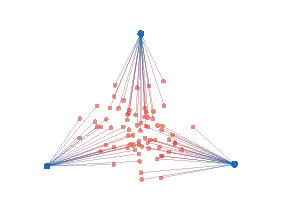
\includegraphics[width=.23\linewidth]{figures/generative-diffusion-versus-ot-2d/ot-rays.pdf} &
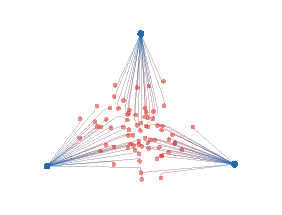
\includegraphics[width=.23\linewidth]{figures/generative-diffusion-versus-ot-2d/schedule-linear.pdf} &
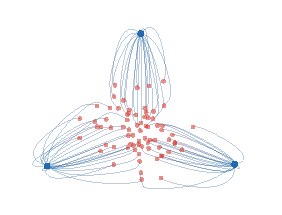
\includegraphics[width=.23\linewidth]{figures/generative-diffusion-versus-ot-2d/schedule-vp.pdf} &
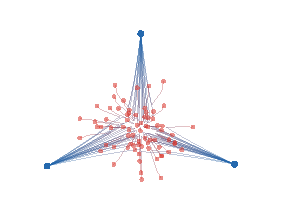
\includegraphics[width=.23\linewidth]{figures/generative-diffusion-versus-ot-2d/schedule-overshoot.pdf}
\end{tabular}}
\caption{\emph{Quadratic-OT rays and exact reverse-flow trajectories for three interpolants.} All four panels use the same three-Dirac target and centered Gaussian source. From left to right: straight displacement rays selected by quadratic OT; the linear bridge $a_t=1-t$, $b_t=t$; the variance-preserving OU bridge $a_\tau=e^{-\tau}$, $b_\tau=\sqrt{1-e^{-2\tau}}$; and the overshooting bridge $a_t=(1-t)(1-2t)$, $b_t=t$. The last bridge is not a time reparametrization of the preceding two and bends the trajectories more strongly.}
\index{Gaussian!mixture}% strictindex
\index{bridge!OU}% strictindex
\index{bridge!variance-preserving}% strictindex
\index{flow!probability ODE}% strictindex
\index{score function}% strictindex
\index{flow!reverse}% strictindex
\label{fig:generative-diffusion-schedule-comparison}
\end{figure}

\paragraph{Stochastic interpolants.}
\index{stochastic!interpolant}% strictindex
\index{latent!variable}% strictindex
\index{flow!probability ODE}% strictindex
The deterministic construction of Definition~\ref{def-deterministic-interpolant} can be enriched by a static Gaussian perturbation whose amplitude varies along the interpolation. In the construction of Albergo, Boffi and Vanden-Eijnden~\cite{Albergo2025StochasticInterpolants}, one auxiliary Gaussian variable is shared by the entire path.
\begin{defn}[Stochastic interpolant]\label{def-stochastic-interpolant}
Let $(X_0,X_1)\sim\pi\in\Couplings(\alpha_0,\alpha_1)$, let $Z\sim\Gaussian(0,\Id)$ be independent of $(X_0,X_1)$, and let $I_t$ be a deterministic interpolant for this coupling. Given an absolutely continuous noise schedule $\gamma:[0,1]\to\RR$ satisfying $\gamma(0)=\gamma(1)=0$, the stochastic interpolant is
\begin{equation}\label{eq-static-noise-stochastic-interpolant}
	X_t=I_t(X_0,X_1)+\gamma(t)Z,
	\qquad \alpha_t=\operatorname{Law}(X_t).
\end{equation}
Assume in addition that $\EE\int_0^1\norm{\partial_tI_t(X_0,X_1)+\dot\gamma(t)Z}^2\,\d t<+\infty$.
\end{defn}
The same draw of $Z$ is used for every $t$: conditionally on $(X_0,X_1,Z)$, the path remains absolutely continuous. Thus~\eqref{eq-static-noise-stochastic-interpolant} is the push-forward construction~\eqref{eq:interp-coupling} with latent variable $u=(X_0,X_1,Z)$. Its Eulerian velocity is
\[
	v_t(x)=\EE\bigl[\partial_tI_t(X_0,X_1)+\dot\gamma(t)Z\mid X_t=x\bigr],
\]
and Proposition~\ref{prop-flow-matching-vector-field} gives the associated continuity equation. When regularity permits their construction, the associated SDEs are alternative dynamics with the same one-time marginals; they are not obtained by replacing $Z$ with independent noise at every time.

\begin{rem}[Brownian realizations of interpolant marginals]\label{rem-noisy-stochastic-interpolants}
\index{stochastic!interpolant}% strictindex
\index{Fokker-Planck@Fokker--Planck!equation}% strictindex
\index{flow!probability ODE}% strictindex
One can instead realize an interpolating marginal curve by Brownian-in-time dynamics. This gives a different path law from Definition~\ref{def-stochastic-interpolant}, although the one-time marginals can coincide, as in Proposition~\ref{prop-static-ou-equivalence}. The static-noise paths are absolutely continuous, whereas nondegenerate diffusion paths have nonzero quadratic variation. Let
\[
	\d X_t=r_t(U,X_t)\d t+\sigma_t(U,X_t)\d B_t,
	\qquad \alpha_t=\operatorname{Law}(X_t),
\]
where $U\sim\pi$ is static and $B_t$ is Brownian motion. Conditioning on the observed state defines
\[
	v_t(x)=\EE\bigl[r_t(U,X_t)\mid X_t=x\bigr],
	\qquad
	D_t(x)=\EE\bigl[\sigma_t(U,X_t)\sigma_t(U,X_t)^\top\mid X_t=x\bigr].
\]
For smooth test functions $\varphi$,
\[
	\frac{\d}{\d t}\int\varphi\d\alpha_t
	=
	\int\dotp{\nabla\varphi}{v_t}\d\alpha_t
	+
	\frac12\int\tr(D_t\nabla^2\varphi)\d\alpha_t,
\]
or, in distributional form,
\begin{equation}\label{eq:noisy-interpolant-fokker-planck}
	\partial_t\alpha_t+\diverg(\alpha_tv_t)
	=
	\frac12\sum_{i,j}\partial_{i,j}^2\bigl((D_t)_{i,j}\alpha_t\bigr).
\end{equation}
The noisy analogue of~\eqref{eq:flow-matching} therefore regresses the drift through $\min_w\EE[\norm{w_t(X_t)-r_t(U,X_t)}^2]$. It learns a Fokker--Planck drift rather than a pure continuity-equation velocity. If $\alpha_t=\rho_t\d x$ has a smooth positive density, the same marginal curve has the formal probability-flow representation $\partial_t\rho_t+\diverg(\rho_t\bar v_t)=0$, where $\bar v_t=v_t-(2\rho_t)^{-1}\diverg(\rho_tD_t)$ and the matrix divergence is taken row-wise. For $D_t=\sigma_t^2\Id$, this becomes $\bar v_t=v_t-(\sigma_t^2/2)\nabla\log\rho_t$.
\index{flow!probability ODE}% strictindex
\end{rem}

% -----------------------------------------------------------------------------

\section{One-Step Generative Models}
\label{sec-one-step-generative-models}
\index{one-step generative model}% strictindex

One-step generative models try to keep the geometric training principle of flows while removing expensive multi-step integration at sampling time. To expose this tradeoff, we first describe direct non-parametric sampling by a Wasserstein flow; the subsequent constructions move that evolution into training and store its endpoint in a single generator evaluation.
\index{generative model}% strictindex

\paragraph{Non-parametric sampling via gradient flow.}
\index{Wasserstein!gradient flow}% strictindex
\index{particle!gradient flow}% strictindex
\index{sliced Wasserstein!flow}% strictindex
Let $\beta$ be the target law and let $\mathcal D$ be a discrepancy that vanishes only on the diagonal. Define
\begin{equation}\label{eq-one-step-discrepancy-energy}
	\mathcal E_\beta(\alpha)\eqdef\mathcal D(\alpha,\beta).
\end{equation}
A direct sampling strategy follows the formal $\Wass_2$ gradient flow
\begin{equation}\label{eq-nonparametric-discrepancy-flow}
	\partial_t\alpha_t+\diverg(\alpha_t v_t)=0,
	\qquad
	v_t=-\Wgrad\mathcal E_\beta(\alpha_t)
	=-\nabla\delta_\alpha\mathcal E_\beta(\alpha_t).
\end{equation}
If this flow is globally well posed and converges to a global minimizer of $\mathcal E_\beta$, then its limit is $\beta$. These are substantial assumptions, not automatic consequences of the definition of a discrepancy. If $\alpha_0=n^{-1}\sum_{i=1}^n\delta_{X_i(0)}$ and the dynamics preserves empirical measures, then~\eqref{eq-nonparametric-discrepancy-flow} becomes the particle system
\begin{equation}\label{eq-nonparametric-particle-flow}
	\dot X_i(t)=v_t(X_i(t))
	=-\Wgrad\mathcal E_\beta(\alpha_t)(X_i(t)),
	\qquad
	\alpha_t=\frac1n\sum_{i=1}^n\delta_{X_i(t)}.
\end{equation}
For fixed $n$, such a curve cannot converge weakly to a non-atomic target while retaining exactly $n$ equally weighted atoms. The sampling interpretation is therefore a large-particle approximation: one evolves a sufficiently rich cloud and lets $n$ increase. This approach is most practical in low dimension because it stores and repeatedly updates many interacting particles, in sharp contrast with flow matching, which learns a field that can subsequently transport arbitrary fresh samples.

A particularly transparent example uses the sliced objective introduced for imaging and barycenters by Rabin, Peyr\'e, Delon and Bernot~\cite{rabin-ssvm-11}: take $\mathcal E_\beta(\alpha)=\frac12\SW_2^2(\alpha,\beta)$, with $\SW_2$ defined in Section~\ref{sec-sliced-wasserstein}. Assume that $\alpha$ has sufficient moments and that its projected laws are atomless, so the projected monotone maps are uniquely defined for $\sigma$-almost every direction. If $T_\theta$ denotes the monotone transport from $(P_\theta)_\sharp\alpha$ to $(P_\theta)_\sharp\beta$, then the formal descent velocity is
\begin{equation}\label{eq-sliced-wasserstein-flow-velocity}
	v_{\SW}[\alpha,\beta](x)
	=
	\int_{\Sphere^{d-1}}
	\big(T_\theta(P_\theta x)-P_\theta x\big)\,\theta\,\d\sigma(\theta).
\end{equation}
Indeed, the spatial derivative of the first variation of $\frac12\Wass_2^2(\alpha,\beta)$ in one dimension is $s-T(s)$; descent reverses this sign, and composition with $P_\theta$ lifts the displacement along $\theta$. Empirical implementations replace the integral by sampled directions and compute each projected displacement by one-dimensional sorting. This is the sliced-Wasserstein flow studied by Cozzi and Santambrogio~\cite{CozziSantambrogio2024SlicedFlow}. For a standard Gaussian target and an initial law with finite entropy and second moment, they prove well-posedness and $\SW_2^2(\alpha_t,\beta)\leq C/t$; their argument extends to isotropic Gaussian covariances but not to arbitrary anisotropic targets. They also show that the limiting characteristic map need not be the optimal transport map. Gaussian closure of this flow is revisited in Section~\ref{sec-gaussian-closure-transport-dynamics} and Proposition~\ref{prop-centered-gaussian-covariance-catalogue}.
\index{Gaussian!closure}% strictindex
\index{monotone!transport map}% strictindex

Figure~\ref{fig:generative-w2-vs-sliced-flow-shapes} contrasts the empirical flow of $\frac12\Wass_2^2(\cdot,\beta)$, for which a fixed optimal assignment gives straight relaxation curves, with the $\Wass_2$ gradient flow of $\frac12\SW_2^2(\cdot,\beta)$, whose projected assignments are recomputed along the evolution.

\begin{figure}[ht]
\centering
{\setlength{\tabcolsep}{.12em}
\begin{tabular}{@{}>{\centering\arraybackslash}m{2.5em}@{\hspace{.15em}}*{6}{>{\centering\arraybackslash}m{.142\linewidth}}@{}}
{\small $\Wass_2$} &
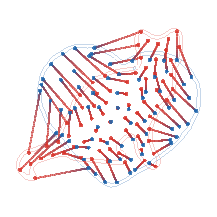
\includegraphics[width=\linewidth]{figures/generative-w2-vs-sliced-flow-shapes/w2-trajectories.pdf} &

\includegraphics[width=\linewidth]{figures/generative-w2-vs-sliced-flow-shapes/w2-density-0.pdf} &
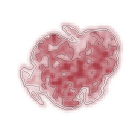
\includegraphics[width=\linewidth]{figures/generative-w2-vs-sliced-flow-shapes/w2-density-1.pdf} &
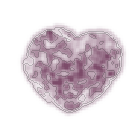
\includegraphics[width=\linewidth]{figures/generative-w2-vs-sliced-flow-shapes/w2-density-2.pdf} &
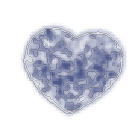
\includegraphics[width=\linewidth]{figures/generative-w2-vs-sliced-flow-shapes/w2-density-3.pdf} &
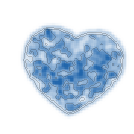
\includegraphics[width=\linewidth]{figures/generative-w2-vs-sliced-flow-shapes/w2-density-4.pdf} \\
{\small $\SW_2$} &
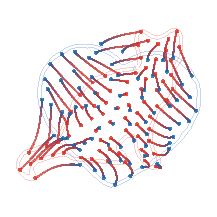
\includegraphics[width=\linewidth]{figures/generative-w2-vs-sliced-flow-shapes/sw-trajectories.pdf} &

\includegraphics[width=\linewidth]{figures/generative-w2-vs-sliced-flow-shapes/sw-density-0.pdf} &
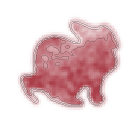
\includegraphics[width=\linewidth]{figures/generative-w2-vs-sliced-flow-shapes/sw-density-1.pdf} &
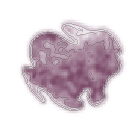
\includegraphics[width=\linewidth]{figures/generative-w2-vs-sliced-flow-shapes/sw-density-2.pdf} &
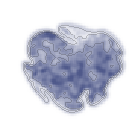
\includegraphics[width=\linewidth]{figures/generative-w2-vs-sliced-flow-shapes/sw-density-3.pdf} &
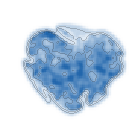
\includegraphics[width=\linewidth]{figures/generative-w2-vs-sliced-flow-shapes/sw-density-4.pdf} \\[-.2em]
& {\small particles} & \multicolumn{5}{c}{\small kernel-density snapshots}
\end{tabular}}
\caption{\emph{Full Wasserstein and sliced-Wasserstein flows from a cat-shaped empirical law to a heart-shaped target.} The left panel in each row shows representative particle trajectories colored from red to blue. The five panels on the right render kernel-density estimates of all particles at common normalized times. The $\Wass_2$ flow follows a fixed optimal assignment and therefore straight relaxation rays, whereas the sliced flow averages one-dimensional sorted rearrangements over projection directions, producing curved trajectories and a different transient density evolution.}
\label{fig:generative-w2-vs-sliced-flow-shapes}
\end{figure}
\index{sliced Wasserstein!flow}% strictindex
\index{kernel!density estimate}% strictindex

\paragraph{One-step models via parameter-domain discrepancy flows.}
\index{one-step generative model}% strictindex
\index{flow!parameter-domain}% strictindex
\index{discrepancy minimization}% strictindex
\index{minibatch bias}% strictindex
\index{parameter space}% strictindex
\index{minibatch}% strictindex
\index{Wasserstein!GAN}% strictindex
\index{MMD-GAN}% strictindex
\index{Sinkhorn!GAN}% strictindex

The most direct one-step strategy is to train the generator parameters themselves by descending the discrepancy~\eqref{eq-one-step-discrepancy-energy}. Let $\zeta$ be a simple latent distribution and let $f_\theta:\Zz\to\Xx$ be a neural generator. The objective is to find $\theta$ such that $(f_\theta)_\sharp\zeta=\beta$, or, in practice, such that the generated law is close to $\beta$. Define
\begin{equation}\label{eq-one-step-parameter-discrepancy}
	H_\beta(\theta)
	\eqdef
	\mathcal E_\beta\big((f_\theta)_\sharp\zeta\big)
	=
	\mathcal D\big((f_\theta)_\sharp\zeta,\beta\big).
\end{equation}
This viewpoint includes Wasserstein GANs, MMD-GANs and Sinkhorn generative models~\cite{WassersteinGAN,MMD-GAN,2017-Genevay-AutoDiff}; when $\mathcal D$ is written through a dual potential or discriminator, it connects directly with the adversarial formulation of Section~\ref{sec-gan-duality}. The resulting training dynamics is the ordinary Euclidean gradient flow in parameter space,
\begin{equation}\label{eq-one-step-parameter-flow}
	\dot\theta_t=-\nabla_\theta H_\beta(\theta_t).
\end{equation}
This parameter flow induces a flow of generated measures, but this induced flow is not intrinsic in general. Set
\[
	\alpha_t\eqdef(f_{\theta_t})_\sharp\zeta,
	\qquad
	X_t=f_{\theta_t}(Z),
	\qquad
	Z\sim\zeta.
\]
\begin{prop}[Velocity induced by a parameter path]\label{prop-parameter-path-continuity}
	Assume that $\Xx=\RR^d$, that $t\mapsto\theta_t$ is continuously differentiable on $[0,T]$, and that, for $\zeta$-almost every $z$, the map $\theta\mapsto f_\theta(z)$ is continuously differentiable. Assume also that $(t,z)\mapsto\partial_\theta f_{\theta_t}(z)$ is jointly measurable and that
	\[
		\int_0^T\!\int_\Zz
		\norm{\partial_\theta f_{\theta_t}(z)\dot\theta_t}
		\,\d\zeta(z)\d t<+\infty.
	\]
	Let $\eta_{t,x}$ be a jointly measurable disintegration of $\d t\,\zeta(\d z)$ under $(t,z)\mapsto(t,f_{\theta_t}(z))$. Then the Eulerian velocity
	\begin{equation}\label{eq-one-step-induced-velocity}
		v_t(x)=\int \partial_\theta f_{\theta_t}(z)\dot\theta_t\,\d\eta_{t,x}(z)
	\end{equation}
		satisfies, in the distributional sense on $(0,T)\times\RR^d$,
	\begin{equation}\label{eq-one-step-induced-continuity}
		\partial_t\alpha_t+\diverg(\alpha_t v_t)=0.
	\end{equation}
	If $\theta_t$ follows~\eqref{eq-one-step-parameter-flow}, then $\dot\theta_t=-\nabla_\theta H_\beta(\theta_t)$ in~\eqref{eq-one-step-induced-velocity}.
\end{prop}

\begin{proof}
	The chain rule gives $\dot X_t=\partial_\theta f_{\theta_t}(Z)\dot\theta_t$. For every bounded measurable $\psi$, disintegration means
	\[
		\int \psi(z)\,\d\zeta(z)=\int_\Xx\left(\int \psi(z)\,\d\eta_{t,x}(z)\right)\d\alpha_t(x)
	\]
	for almost every $t$. Consequently, for every smooth compactly supported $\varphi$,
	\[
		\frac{\d}{\d t}\int \varphi(x)\,\d\alpha_t(x)
		=
		\int \dotp{\nabla\varphi(x)}{v_t(x)}\,\d\alpha_t(x),
	\]
	which is the weak form of~\eqref{eq-one-step-induced-continuity}.
\end{proof}

The velocity~\eqref{eq-one-step-induced-velocity} depends on the parameter value $\theta_t$ and on the latent disintegration, not only on the measure $\alpha_t$. If the parametrization is non-identifiable, two different parameters can generate the same measure while inducing different velocities. Thus~\eqref{eq-one-step-parameter-flow} is a Euclidean gradient flow on parameter space, and only after push-forward a model-dependent flow on measures.
\index{continuity equation}% strictindex
\index{disintegration}% strictindex
\index{generator manifold}% strictindex
A practical difficulty is computing the gradient of $H_\beta$ from samples. One typically uses the minibatch law $\hat\beta_n=n^{-1}\sum_{i=1}^n\de_{Y_i}$, where $Y_i\overset{\mathrm{i.i.d.}}{\sim}\beta$, and replaces $H_\beta$ by the random objective $H_{\hat\beta_n}$. Unlike standard stochastic-gradient constructions, this substitution is not generally unbiased for nonlinear discrepancies:
\[
	\EE\left[\nabla_\theta H_{\hat\beta_n}(\theta)\right]
	\neq
	\nabla_\theta H_\beta(\theta).
\]
The expectation is over the data minibatch. This bias is a finite-sample effect of inserting the empirical measure inside a nonlinear transport or adversarial optimization before differentiating; it is distinct from the optimization noise of stochastic gradient descent. MMD losses admit unbiased $U$-statistic variants, but OT and entropic OT objectives generally exhibit the bias--variance phenomena discussed in Section~\ref{sec-bias-variance-ot}.
\index{stochastic!gradient}% strictindex
\index{finite-sample bias}% strictindex
\index{empirical!measure}% strictindex
\index{Sinkhorn!divergence}% strictindex

\paragraph{One-step models from Wasserstein flows.}
\index{Wasserstein!flow of discrepancy}% strictindex
\index{natural gradient}% strictindex
\index{flow!one-step}% strictindex
\index{Wasserstein!gradient flow}% strictindex

This construction keeps the same discrepancy but changes the geometry of descent. Instead of following its Euclidean gradient in parameter space, one approximates the intrinsic flow~\eqref{eq-nonparametric-discrepancy-flow} and fits each distribution-space update by a generator. This natural-gradient-type dynamics is less tied to a particular parametrization, although its convergence still depends on the geometry of $\mathcal E_\beta$.

Let $\zeta$ be a simple latent distribution and let $\alpha_\theta=(G_\theta)_\sharp\zeta$ be the model distribution. Typical choices for $\mathcal E_\beta$ include a smoothed relative entropy, an MMD/IPM loss, or the debiased Sinkhorn divergence $\bar\MK_\c^\epsilon(\alpha,\beta)$ introduced in Section~\ref{sec-sinkhorn-div}. Writing its formal Wasserstein descent as
\index{maximum mean discrepancy}% strictindex
\index{integral probability metric}% strictindex
\index{Sinkhorn!divergence}% strictindex
\begin{equation}\label{eq-one-step-wgf}
	\partial_t\al_t+\diverg(\al_t v_t)=0,
	\qquad
	v_t(x)=-\Wgrad\mathcal E_\beta(\al_t)(x)
	=-\nabla\delta_\alpha \mathcal E_\beta(\al_t)(x),
\end{equation}
one fits, at each training time $t$, a parametric residual field $U_{\eta_t}$ along the current model distribution:
\begin{equation}\label{eq-one-step-l2-fit}
	\min_\eta \int
		\norm{U_\eta(x)-v_t(x)}^2
		\,\d\al_t(x).
\end{equation}
In a particle or generator implementation, the learned residual is then used to update the current generator by
\[
	\alpha_{\theta}^{+}
	=
	(\Id+\tau U_{\eta_t})_\sharp \alpha_\theta,
	\qquad\text{or equivalently}\qquad
	G_\theta^{+}(z)=G_\theta(z)+\tau U_{\eta_t}(G_\theta(z)).
\]
This is an ideal function-space update. If the residuals were stored as a growing composition, evaluation would still require one layer per training update and the model would not be one-step. A genuine one-step implementation therefore fits the updated outputs back into a fixed generator architecture, or distills the accumulated transport into one network, so that the final sampler remains a single evaluation of $G_\theta$.


After many training updates, the fixed-architecture or distilled generator is evaluated once at test time. W-Flow follows this principle with the Sinkhorn divergence as a tractable global discrepancy~\cite{Han2026WFlow}. Related entropic constructions use Sinkhorn-type discrepancies to define the distribution-space flow~\cite{He2026SinkhornDrifting}. The drifting models discussed below retain the fit-and-distill mechanism but prescribe a cheaper field that need not be an exact Wasserstein gradient.
\index{Wasserstein!gradient}% strictindex
\index{gradient!flow}% strictindex
\index{Wasserstein!gradient flow}% strictindex
\index{Sinkhorn!divergence}% strictindex
\index{drifting!model}% strictindex

\paragraph{Stein variational gradient descent.}\label{sec-svgd-generative-flow}
\index{Stein variational gradient descent@Stein variational gradient descent (SVGD)}% strictindex
\index{gradient!kernelized flow}% strictindex
\index{Stein force}% strictindex
\index{Benamou-Brenier@Benamou--Brenier!kernelized}% strictindex
\index{Stein operator}% strictindex
\index{kernelized Stein discrepancy}% strictindex
SVGD is not the ordinary $\Wass_2$ gradient flow of $\KL(\alpha|\beta)$. It replaces the $L^2(\alpha)$ tangent geometry by a kernel-smoothed Stein geometry whose admissible velocities lie in a vector-valued RKHS; this is closely related to the kernelized Benamou--Brenier geometry of Section~\ref{sec-kernelized-bb-distance}. Its original motivation is Bayesian sampling: the target $\beta=\rho_\beta\,\d x$ is known through its score $\nabla\log\rho_\beta$, but not necessarily through its normalizing constant, and one seeks to transport particles without estimating the score of their empirical law~\cite{LiuWang2016SVGD}.

\begin{defn}[SVGD vector field]\label{def-svgd-vector-field}
Let $\beta=\rho_\beta\d x$, where $\rho_\beta$ is positive and continuously differentiable. Let $k$ be a continuously differentiable positive-definite kernel with scalar RKHS $\RKHS_k$, and assume that its first-derivative evaluations are bounded on $\RKHS_k$. If the $\RKHS_k^d$-valued map $y\mapsto k(y,\cdot)\nabla\log\rho_\beta(y)+\nabla_yk(y,\cdot)$ is Bochner integrable under $\alpha$, the SVGD field is the unique minimizer
\begin{equation}\label{eq-svgd-local-problem}
	v_\alpha^{\mathrm{SVGD}}
	\eqdef
	\uargmin{v\in\RKHS_k^d}
	\left\{
		-\int\!\bigl(\dotp{\nabla\log\rho_\beta(x)}{v(x)}+\diverg v(x)\bigr)\,\d\alpha(x)
		+\frac12\norm{v}_{\RKHS_k^d}^2
	\right\}.
\end{equation}
By the reproducing property, it has the explicit form
\begin{equation}\label{eq-svgd-velocity}
	v_{\alpha}^{\mathrm{SVGD}}(x)
	=
	\int
	\Big(k(y,x)\nabla\log\rho_\beta(y)+\nabla_y k(y,x)\Big)
	\d\alpha(y).
\end{equation}
\end{defn}
For smooth positive $\alpha$, under the usual Stein boundary condition, the linear term in~\eqref{eq-svgd-local-problem} is the directional derivative of $\KL(\cdot|\beta)$ along $(\Id+s v)_\sharp\alpha$. Unlike that density-level expression, the right-hand side of~\eqref{eq-svgd-velocity} remains meaningful for empirical $\alpha$.
\eqllead{Thus}{eq-svgd-mean-field}{
	\partial_t\alpha_t+\diverg\bigl(\alpha_t v_{\alpha_t}^{\mathrm{SVGD}}\bigr)=0.
}
For particles $\alpha_n^{(\ell)}=n^{-1}\sum_i\delta_{X_i^{(\ell)}}$, this becomes the explicit update
\begin{equation}\label{eq-svgd-particle-update}
	X_i^{(\ell+1)}
	=
	X_i^{(\ell)}
	+
	\tau\,\frac{1}{n}\sum_{j=1}^n
	\Big(k(X_j^{(\ell)},X_i^{(\ell)})\nabla\log\rho_\beta(X_j^{(\ell)})
	+
		\nabla_1k(X_j^{(\ell)},X_i^{(\ell)})\Big).
\end{equation}
The first term attracts particles toward increasing target log-density; while particles remain distinct, the second counteracts concentration through kernel repulsion. For translation-invariant radial kernels, this repulsion vanishes after exact coalescence and is therefore not an unconditional anti-collapse guarantee. The analyses in~\cite{Liu2017SVGDGradientFlow,DuncanNueskenSzpruch2019SVGDGeometry,NueskenRenger2021SVGDAsymptotics} make precise its gradient-flow interpretation and its many-particle behavior. SVGD is close in spirit to the drifting fields below, but its velocity is the closed-form RKHS steepest-descent field rather than a prescribed field subsequently fitted by regression.

Figure~\ref{fig:generative-w2-vs-svgd-entropy-flow} contrasts this RKHS flow with a particle closure of the Wasserstein gradient flow of \(\KL(\alpha|\beta)\). The latter evaluates the current score \(\nabla\log\rho_\alpha\) by a Gaussian KDE, while SVGD avoids this density estimate and uses the target score together with a kernel repulsion.
\begin{figure}[H]
\centering
\begin{tabular}{@{}>{\centering\arraybackslash}m{.47\linewidth}@{\hspace{.03\linewidth}}>{\centering\arraybackslash}m{.47\linewidth}@{}}
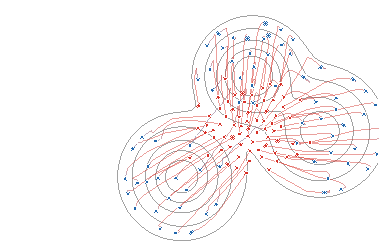
\includegraphics[width=\linewidth]{figures/generative-w2-vs-svgd-entropy-flow/w2-kde-trajectories.pdf} &
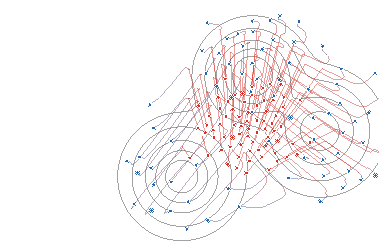
\includegraphics[width=\linewidth]{figures/generative-w2-vs-svgd-entropy-flow/svgd-trajectories.pdf} \\[-.1em]
{\small $\Wass_2$ KDE closure} & {\small SVGD}
\end{tabular}
\caption{\emph{Particle trajectories for two deterministic descents of relative entropy.} Both descents target the same three-Gaussian density, shown by gray contours. The left panel approximates the \(\Wass_2\) gradient flow of \(\KL(\alpha|\beta)\) by the KDE velocity \(\nabla\log\rho_\beta-\nabla\log\rho_{\alpha,h}\). The right panel uses the RBF-kernel SVGD velocity~\eqref{eq-svgd-velocity}, where target-score attraction is coupled with RKHS repulsion. Both panels use the same initial particles and color trajectory time from red to blue.}
\label{fig:generative-w2-vs-svgd-entropy-flow}
\end{figure}
\index{Stein variational gradient descent@Stein variational gradient descent (SVGD)}% strictindex
\index{Fokker--Planck particle closure}% strictindex

\paragraph{Drifting flows.}
\index{drifting!field}% strictindex

Computing the exact velocity in~\eqref{eq-one-step-wgf} can be costly. Drifting methods instead prescribe a cheaper distribution-correcting field, typically combining attraction toward the data with a self-normalization term, and regress it in $L^2(\al_t)$ as in~\eqref{eq-one-step-l2-fit}~\cite{Deng2026Drifting,Gretton2026DriftingWGF}. Such a field need not be the Wasserstein gradient of a fixed discrepancy. A simple continuous construction uses a strictly positive kernel $K_\epsilon(x,y)$ for which the following integrals are finite and defines, for every probability measure $\nu$,
\index{Wasserstein!gradient}% strictindex
\index{kernel!positive}% strictindex
\begin{equation}\label{eq-normalized-kernel-drift}
	B_\epsilon[\nu](x)
	\eqdef
	\frac{\int (y-x)K_\epsilon(x,y)\,\d\nu(y)}
	     {\int K_\epsilon(x,y)\,\d\nu(y)}.
\end{equation}
For the Gaussian kernel
\index{kernel!Gaussian}% strictindex
$K_\epsilon(x,y)=\exp(-\norm{x-y}^2/(2\epsilon))$, this normalized field is a score of a smoothed density:
\index{score function}% strictindex
\begin{equation}\label{eq-normalized-kernel-score}
	B_\epsilon[\nu](x)
	=
	\epsilon\nabla\log\!\left(\int K_\epsilon(x,y)\,\d\nu(y)\right).
\end{equation}
The drifting velocity is
\begin{equation}\label{eq-cross-minus-self-drift}
	v_t(x)=B_\epsilon[\beta](x)-B_\epsilon[\al_t](x)
	=
	\epsilon\nabla\log
	\frac{\int K_\epsilon(x,y)\,\d\beta(y)}
	     {\int K_\epsilon(x,y)\,\d\al_t(y)}.
\end{equation}
The first term pulls samples toward data, while the second acts as a repulsive correction before coalescence. If all empirical particles occupy the same point, their self displacement is zero and they all receive the same target drift, so this deterministic field cannot recreate diversity. For fixed $\nu$, $B_\epsilon[\nu]$ is the Gaussian mean-shift displacement in~\eqref{eq-l2-attention-mean-shift}: it points from $x$ toward the local kernel barycenter of $\nu$. Thus~\eqref{eq-cross-minus-self-drift} subtracts the current model's mean-shift field from the target field.

Sampling follows the usual continuity equation $\partial_t\al_t+\diverg(\al_t v_t)=0$ from a prescribed simple law $\al_{t=0}=\al_0$; equivalently, particles solve $\dot X_i(t)=v_t(X_i(t))$. A direct implementation repeatedly evaluates~\eqref{eq-cross-minus-self-drift}. In a one-step implementation, the field is instead regressed by a neural network through~\eqref{eq-one-step-l2-fit}, and the accumulated evolution is fitted or distilled into the generator as described above. This moves the repeated integration cost from inference to training.
\index{kernel!norm}% strictindex


Figure~\ref{fig:generative-drifting-model-trajectories} gives a schematic comparison of two attraction-minus-weighted-self constructions; because several numerical choices differ, it should not be read as isolating the causal effect of one term.

\begin{figure}[ht]
\centering
\begin{tabular}{@{}cc@{}}
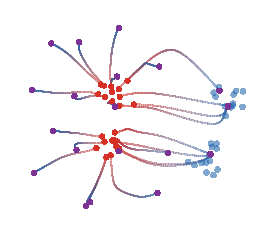
\includegraphics[width=.38\linewidth]{figures/generative-drifting-model-trajectories/unnormalized-trajectories.pdf} &
\index{drifting!model}% strictindex
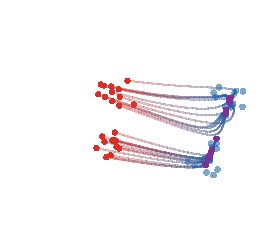
\includegraphics[width=.38\linewidth]{figures/generative-drifting-model-trajectories/normalized-trajectories.pdf}
\\[-.1em]
\small unnormalized Gaussian drift & \small normalized Gaussian drift
\index{self-corrected field}% strictindex
\end{tabular}
\caption{\emph{Two schematic Gaussian-kernel drifting trajectories for a small particle generator.} Both panels use attraction-minus-weighted-self fields. The left uses unnormalized Gaussian averages; the right uses normalized Gaussian mean-shift averages. Their target and self bandwidths, self weights, integration horizons and step sizes differ, and both simulations cap the instantaneous speed. The display compares two tuned constructions rather than a controlled ablation of self-repulsion.}
\label{fig:generative-drifting-model-trajectories}
\end{figure}

\section{Moment Measures}
\label{sec-moment-measures}
\index{moment measure}% strictindex
\index{convex!potential}% strictindex

Moment measures give another way to make a whole distribution from one convex potential. Instead of first fixing a simple source law and then learning a transport map, one asks for a convex function whose own log-concave density is pushed forward by its gradient. This couples sampling and mapping in a rigid way: the same potential defines both the source density and the Brenier map. The reward is a hidden convex structure: after a suitable optimal-transport reformulation, a nonlinear equation on convex functions becomes a convex minimization problem for probability densities. This is one of the cleanest places where optimal transport, Pr\'ekopa-type inequalities and convex geometry meet.
\index{log-concave!density}% strictindex
\index{displacement convexity}% strictindex

\begin{defn}[Moment measure of a convex function]\label{def-moment-measure}
\index{convex!function}% strictindex
	Let $u:\RR^d\to\RR\cup\{+\infty\}$ be a proper lower-semicontinuous convex function such that $0<Z_u\eqdef \int_{\RR^d} e^{-u(x)}\,\d x <+\infty$. The normalized log-concave measure associated with $u$ is $\eta_u \eqdef Z_u^{-1} e^{-u(x)}\,\d x$.
	These assumptions force the effective domain of $u$ to have nonempty interior, so convex differentiability implies that $\nabla u$ exists $\eta_u$-almost everywhere. The moment measure of $u$ is
\index{moment measure}% strictindex
	\[
		\mathfrak M(u)\eqdef (\nabla u)_\sharp \eta_u.
	\]
\end{defn}

The normalization removes additive constants in $u$. Translations of the argument are another invariance: if $u_a(x)=u(x-a)$, then $\eta_{u_a}$ is the translate of $\eta_u$, while $\nabla u_a(x)=\nabla u(x-a)$, hence $\mathfrak M(u_a)=\mathfrak M(u)$. A first obstruction is immediate. Formally, if $u$ is smooth and $e^{-u}$ decays fast enough for the boundary term to vanish, then
\[
	\int y\,\d\mathfrak M(u)(y)
	=
	Z_u^{-1}\int \nabla u(x)e^{-u(x)}\,\d x
	=
	-Z_u^{-1}\int \nabla(e^{-u(x)})\,\d x
	=0.
\]
Thus moment measures are necessarily centered. The nonsmooth theory uses essentially continuous convex functions: these are lower-semicontinuous convex functions whose set of discontinuity points has zero $\mathcal H^{d-1}$ measure. Since a convex function is continuous in the interior of its effective domain, this condition controls only its boundary behavior.
\index{moment measure}% strictindex
\index{essential continuity}% strictindex
\index{barycenter}% strictindex

Figure~\ref{fig:moment-measure-forward-map} shows the forward construction in one dimension. The map $u'$ is implicit in the push-forward, but the display focuses on the two visible measures: the log-concave source $\eta_u=Z_u^{-1}e^{-u}\d x$ and the resulting moment measure $\mathfrak M(u)$.

\begin{figure}[ht]
\centering
\begin{tabular}{@{}ccc@{}}
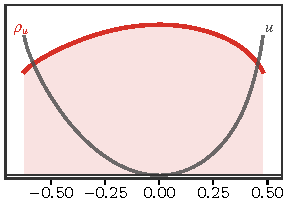
\includegraphics[width=.30\linewidth]{figures/moment-measure-forward-map/slanted-source.pdf} &
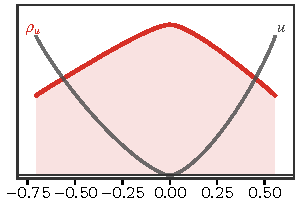
\includegraphics[width=.30\linewidth]{figures/moment-measure-forward-map/twobump-source.pdf} &
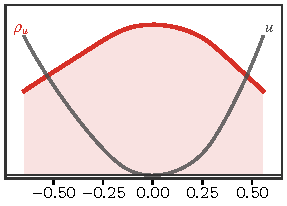
\includegraphics[width=.30\linewidth]{figures/moment-measure-forward-map/threebump-source.pdf} \\[-.2em]
{\small $u$ and $\eta_u$} &
{\small $u$ and $\eta_u$} &
{\small $u$ and $\eta_u$} \\[.35em]
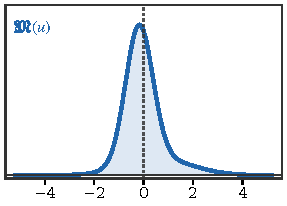
\includegraphics[width=.30\linewidth]{figures/moment-measure-forward-map/slanted-moment.pdf} &
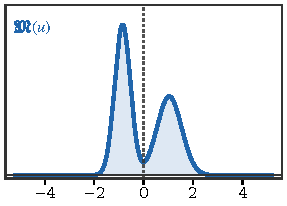
\includegraphics[width=.30\linewidth]{figures/moment-measure-forward-map/twobump-moment.pdf} &
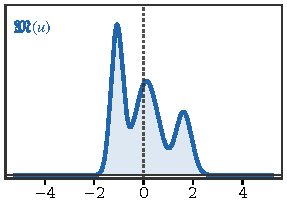
\includegraphics[width=.30\linewidth]{figures/moment-measure-forward-map/threebump-moment.pdf} \\[-.2em]
{\small slanted unimodal $\mathfrak M(u)$} &
{\small two-bump $\mathfrak M(u)$} &
{\small three-bump $\mathfrak M(u)$}
\end{tabular}
\caption{\emph{Forward moment-measure construction in one dimension.} Each column shows a convex potential $u$ chosen so that the moment measure has a prescribed shape: a skewed unimodal density, two bumps, and three bumps with different widths and heights. The top row overlays $u$ (gray, vertically rescaled) with the density of the log-concave source $\eta_u=Z_u^{-1}e^{-u}\d x$ (red), while the bottom row shows $\mathfrak M(u)=(u')_\sharp\eta_u$ (blue); the dashed vertical line marks the zero barycenter.}
\label{fig:moment-measure-forward-map}
\end{figure}

\begin{thm}[Cordero--Erausquin--Klartag]\label{thm-moment-measure-characterization}
\index{moment measure}% strictindex
\index{barycenter}% strictindex
	Let $\al\in\Pp_1(\RR^d)$ be a probability measure. There exists an essentially continuous convex function $u$ such that $\al=\mathfrak M(u)$ if and only if
	\[
		\int y\,\d\al(y)=0
		\qquad\text{and}\qquad
		\supp(\al)\text{ is not contained in a hyperplane.}
	\]
	Under these conditions, $u$ is unique up to translations of the argument and additive constants.
\end{thm}

This theorem is due to Cordero--Erausquin and Klartag~\cite{CorderoErausquinKlartag2015MomentMeasures}. It is a functional analogue of a Minkowski-type problem: the target measure prescribes how the gradient image of a log-concave density should be distributed. The hyperplane condition is the natural non-degeneracy assumption; otherwise the prescribed gradient image lives in a lower-dimensional affine direction and no coercive full-dimensional convex potential can be recovered.
\index{Minkowski problem}% strictindex
\index{log-concave!measure}% strictindex

\begin{example}[Quadratic potentials]\label{ex-moment-measure-gaussian}
\index{Gaussian!measure}% strictindex
\index{moment measure}% strictindex
	Let $A\in\RR^{d\times d}$ be symmetric positive definite and $u(x)=\frac12 x^\top A x + c$. Then $\eta_u=\Nn(0,A^{-1})$ and $\nabla u(x)=Ax$, so $\mathfrak M(u)=\Nn(0,A)$.
	Thus centered non-degenerate Gaussians are moment measures. This example also shows the self-dual flavor of the construction: the covariance of the log-concave source is inverted by the linear gradient map.
\index{moment measure}% strictindex
\end{example}

\paragraph{Optimal-transport variational formulation.}
\index{maximal correlation}% strictindex
\index{entropy}% strictindex
Santambrogio~\cite{Santambrogio2015MomentMeasures} reformulates the moment-measure problem as a minimization over absolutely continuous probability measures. For a centered $\al\in\Pp_1(\RR^d)$, define the maximal-correlation transport functional, with values in $\RR\cup\{+\infty\}$,
\begin{equation}\label{eq-moment-max-correlation}
	\mathsf{MC}_\al(\eta)
	\eqdef
	\sup_{\pi\in\Couplings(\eta,\al)}
	\int_{\RR^d\times\RR^d} x\cdot y\,\d\pi(x,y).
\end{equation}
By Kantorovich duality for the scalar-product cost,
\begin{equation}\label{eq-moment-max-correlation-dual}
	\mathsf{MC}_\al(\eta)
	=
	\inf_{v\ \mathrm{convex}}
	\left\{
		\int v(x)\,\d\eta(x)+\int v^*(y)\,\d\al(y)
	\right\},
\end{equation}
where the infimum is over convex functions for which both integrals are well defined and $v^*$ is the Legendre transform. If $\eta,\al\in\Pp_2(\RR^d)$, then
\index{Legendre transform}% strictindex
\begin{equation}\label{eq-moment-correlation-w2}
	\mathsf{MC}_\al(\eta)
	=
	\frac12\int \norm{x}^2\,\d\eta(x)
	+
	\frac12\int \norm{y}^2\,\d\al(y)
	-
	\frac12\Wass_2^2(\eta,\al).
\end{equation}
The variational problem attached to a centered target $\al$ is
\begin{equation}\label{eq-moment-measure-variational}
	\min_{\eta\in\Pp_1(\RR^d)}
	\left\{
		\mathcal H(\eta)+\mathsf{MC}_\al(\eta)
	\right\},
	\qquad
		\mathcal H(r\,\d x)\eqdef \int r(x)\log r(x)\,\d x,
\end{equation}
where $\mathcal H$ is the relative entropy with respect to Lebesgue measure, in the sigma-finite-reference convention corresponding to the KL divergence of Definition~\ref{def-measure-relative-entropy}; set $\mathcal H(\eta)=+\infty$ when $\eta$ is not absolutely continuous.
The centering of $\al$ makes this functional invariant under translations of $\eta$, since translating $\eta$ by a vector $a$ changes $\int x\cdot y\,\d\pi$ by $a\cdot\int y\,\d\al(y)=0$.
\index{Kantorovich!duality}% strictindex
\index{Legendre transform}% strictindex
\index{Wasserstein!distance}% strictindex

\begin{prop}[Variational characterization of moment measures]\label{prop-moment-hidden-convexity}
\index{moment measure}% strictindex
\index{hidden convexity}% strictindex
\index{displacement convexity}% strictindex
	Let $\al\in\Pp_1(\RR^d)$ be centered and not supported on a hyperplane. Then the minimization problem~\eqref{eq-moment-measure-variational} admits a solution, unique up to translations. Every minimizer is a probability measure with log-concave density $\eta=Z_u^{-1}e^{-u}\,\d x$, where $u$ is convex, essentially continuous, and satisfies the moment-measure equation $\al=(\nabla u)_\sharp \eta$.
	Conversely, any essentially continuous convex $u$ satisfying this equation yields a global minimizer. If $\al\in\Pp_2(\RR^d)$, the objective $\eta\mapsto\mathcal H(\eta)+\mathsf{MC}_\al(\eta)$ is displacement convex along $\Wass_2$ geodesics of absolutely continuous measures in $\Pp_2(\RR^d)$ whenever the terms are finite. When merely $\al\in\Pp_1(\RR^d)$, the maximal-correlation term remains convex along such finite-second-moment geodesics by approximation; existence and uniqueness on the full $\Pp_1$ domain follow from the lower-semicontinuity argument of Santambrogio.
\end{prop}

\begin{proof}
	The existence proof has two ingredients. First, since $\al$ is centered, translating $\eta$ does not change either $\mathcal H(\eta)$ or $\mathsf{MC}_\al(\eta)$, so one can center a minimizing sequence. Second, the assumption that $\al$ is not supported on a hyperplane gives a coercive lower bound of the form $\mathsf{MC}_\al(\eta)\geq c_\al\int\norm{x}\,\d\eta(x)$ for centered absolutely continuous $\eta$, with $c_\al>0$. Together with the lower-semicontinuity estimates for entropy and maximal correlation, this yields a minimizer~\cite{Santambrogio2015MomentMeasures}.

	Let $\eta=r\,\d x$ be a minimizer and let $u$ be a convex optimizer in the dual formula~\eqref{eq-moment-max-correlation-dual}. Keeping $u$ fixed and varying $\eta$ in~\eqref{eq-moment-measure-variational} gives the Euler equation
	\[
		\log r(x)+1+u(x)=\mathrm{constant}
		\qquad\text{on }\{r>0\},
	\]
	so $\eta=Z_u^{-1}e^{-u}\d x$. The optimality condition for the scalar-product transport problem says that an optimal coupling is supported on $\{(x,y):y\in\partial u(x)\}$. Since $\eta$ is absolutely continuous and $u$ is convex, $\partial u(x)=\{\nabla u(x)\}$ for $\eta$-almost every $x$, hence $\al=(\nabla u)_\sharp\eta$.

	Conversely, add a constant to \(u\) so that \(\eta=e^{-u}\d x\), and first let \(\nu\in\Pp_2(\RR^d)\) be compactly supported. Write \(T=\nabla v\) for the Brenier map from \(\eta\) to \(\nu\), and \(\eta_t=((1-t)\Id+tT)_\sharp\eta\). Denote the lower right derivative of the objective along this geodesic by
	\[
		D^+\!\left(\mathcal H+\mathsf{MC}_\al\right)(\eta;\nu)
		\eqdef
		\liminf_{t\downarrow0}
		\frac{(\mathcal H+\mathsf{MC}_\al)(\eta_t)-(\mathcal H+\mathsf{MC}_\al)(\eta)}{t}.
	\]
	The nonsmooth one-sided estimate of~\cite{Santambrogio2015MomentMeasures} is
	\[
		D^+\!\left(\mathcal H+\mathsf{MC}_\al\right)(\eta;\nu)
		\geq
		-\int(\Delta^{\mathrm{ac}}v-d)\,\d\eta
		+\int\dotp{\nabla v-x}{\nabla u}\,\d\eta,
	\]
	where \(\Delta^{\mathrm{ac}}v\) is the Lebesgue density of the absolutely continuous part of the distributional Laplacian of the convex potential \(v\). Essential continuity gives the boundary inequality
	\(\int\dotp{x}{\nabla u}\,\d\eta\leq d\), and therefore
	\[
		D^+\!\left(\mathcal H+\mathsf{MC}_\al\right)(\eta;\nu)
		\geq
		-\int\Delta^{\mathrm{ac}}v\,\d\eta
		+\int\dotp{\nabla v}{\nabla u}\,\d\eta.
	\]
	The distributional Hessian of the convex function \(v\) is a positive matrix-valued measure, so
	\(\Delta v=\Delta^{\mathrm{ac}}v\,\d x+\Delta^s v\) with \(\Delta^s v\geq0\). Since \(\nabla u\,e^{-u}=-\nabla(e^{-u})\), cutoff integration by parts yields
	\[
		-\int\Delta^{\mathrm{ac}}v\,e^{-u}\d x
		-\int\dotp{\nabla v}{\nabla(e^{-u})}\d x
		\geq
		-\int e^{-u}\,\d(\Delta v)
		-\int\dotp{\nabla v}{\nabla(e^{-u})}\d x
		=0.
	\]
	Here boundedness of \(\nabla v\), integrability of \(\nabla(e^{-u})\), and the decay of the nondegenerate log-concave density make the cutoff boundary term vanish. Thus every such one-sided derivative is nonnegative. Displacement convexity gives global minimality against compactly supported competitors, and the approximation theorem in~\cite{Santambrogio2015MomentMeasures} extends it to the full \(\Pp_1\) domain. The equality case in the displacement-convexity argument yields uniqueness modulo translations; this is precisely the unavoidable invariance because translating \(\eta\) does not change \(\mathsf{MC}_\al\) when \(\al\) is centered.

	It remains to justify the convexity assertion. The entropy term is displacement convex by McCann's theorem, recalled in Theorem~\ref{thm-mccann-internal-energy}. If $\al$ has finite second moment, identity~\eqref{eq-moment-correlation-w2} writes $\mathsf{MC}_\al$ as the sum of the $1$-convex moment term $\eta\mapsto\frac12\int\norm{x}^2\,\d\eta$ and the $(-1)$-convex term $\eta\mapsto-\frac12\Wass_2^2(\eta,\al)$, hence $\mathsf{MC}_\al$ is displacement convex. For a target with only a finite first moment, Santambrogio obtains the same convexity along $\Pp_2$ geodesics by approximation and proves the full variational characterization by lower semicontinuity.
\end{proof}

\begin{rem}[Where the convexity is hidden]\label{rem-moment-hidden-convexity}
\index{Toland duality}% strictindex
\index{Prekopa@Pr\'ekopa!inequality}% strictindex
	If one eliminates $\eta$ first, the problem becomes the convex-potential functional
	\[
		u\mapsto
		\int u^*(y)\,\d\al(y)
		-
		\log\!\left(\int e^{-u(x)}\,\d x\right).
	\]
	This is a Toland-type duality: the functional is not visibly convex as a function of $u$, because the first term is convex while the logarithmic partition term is concave in this parametrization. Cordero--Erausquin and Klartag make the hidden convexity visible by changing variables to the dual potential $\varphi=u^*$. Since $u=\varphi^*$ for closed convex potentials, the same functional becomes
	\[
		\varphi\mapsto
		\int \varphi(y)\,\d\al(y)
		-
		\log\!\left(\int e^{-\varphi^*(x)}\,\d x\right).
	\]
	The first term is now affine in $\varphi$. The core Pr\'ekopa--Leindler input is that
	$\varphi\mapsto \log\int e^{-\varphi^*}$ is concave along convex combinations of convex functions; equivalently, the negative log-partition in the display is convex. Santambrogio's formulation reveals the same mechanism in transport language: the difficult convexity becomes the displacement convexity of an entropy-plus-maximal-correlation functional in the measure variable $\eta$.
\end{rem}

\paragraph{Conjugate moment measures for generation.}
\index{log-concave generator}% strictindex
\index{convex!potential generator}% strictindex
\index{generative model}% strictindex
\index{input-convex neural network}% strictindex
\index{conjugate moment measure}% strictindex
\index{moment measure}% strictindex
The moment-measure factorization suggests a generative recipe: sample $X$ from the log-concave law $Z_u^{-1}e^{-u}$ and output $\nabla u(X)$. This ties sampling and mapping through the same convex potential. Vesseron, B\'ethune and Cuturi~\cite{VesseronBethuneCuturi2025ConjugateMomentMeasures} argue that this direct factorization can be poorly adapted to practical generative modeling. Their existence theorem assumes that the target \(\beta\) is absolutely continuous and supported on a compact convex set; under these hypotheses they propose the conjugate factorization
\begin{equation}\label{eq-conjugate-moment-measure}
	\beta
	=
	(\nabla w^*)_\sharp
	\left(Z_w^{-1}e^{-w(z)}\,\d z\right).
\end{equation}
Here $\nabla w^*$ is the Brenier map from the learned absolutely continuous log-concave source to the target distribution $\beta$. This keeps the single-convex-potential philosophy, but places the transport map on the conjugate side; it can be parameterized by input-convex neural networks and trained using OT solvers. For targets outside the theorem's scope, the same expression is a modeling ansatz rather than a general existence statement. From the viewpoint of this chapter, moment measures are therefore a rigorous convex-analytic prototype for one-step generators based on gradients of convex potentials.
\index{Brenier!map}% strictindex
\index{one-step generative model}% strictindex
\index{convex!conjugate}% strictindex

\section{Evolution in Depth of Transformers}
\label{sec-transformer-depth-evolution}
\index{transformer}% strictindex
\index{depth evolution}% strictindex

Deep residual architectures can be read as time discretizations of ODEs or PDEs. For transformers, the transported objects are contextual token representations across depth, not independent generated samples across sampling time. The velocity is induced by attention with weights fixed for this forward analysis; training those weights is a separate evolution.
\index{attention}% strictindex
\index{token measure}% strictindex

Discrete self-attention, its permutation equivariance and its mean-field extension were introduced in the paragraph ``Mean-field attention'' of Section~\ref{sec-measure-to-measure-maps}; see Definition~\ref{def-mean-field-attention-map}. Here the number of tokens is fixed in the discrete model and the limit concerns depth: the number \(T\) of residual attention layers grows while each layer makes an update of size \(1/T\), as in continuous-depth neural networks~\cite{Chen2018NeuralODE}. This is distinct from the many-token limit discussed around Definition~\ref{def-mean-field-attention-map}. Since the attention weights are normalized using the whole current token law, the resulting velocity is nonlinear and context dependent. Related continuous-depth and Sinkhorn-normalized dynamics are studied in~\cite{Sander2022Sinkformers,Castin2025DynamicsTransformers}.
\index{continuous-depth neural network}% strictindex
\index{empirical!context}% strictindex
\index{attention!operator}% strictindex
\index{infinite-depth limit}% strictindex
\index{token limit}% strictindex
\index{transformer}% strictindex
\index{mean-field limit}% strictindex
\index{continuous!depth}% strictindex

We focus on the non-causal single-head mechanism of~\eqref{eq-discrete-self-attention}, ignoring MLP layers, layer normalization and masking. This stripped-down framework isolates the transport structure of a residual attention block.
\index{attention!single-head}% strictindex
\index{layer normalization}% strictindex
\index{causality}% strictindex
\index{masking}% strictindex
\index{transformer}% strictindex

\paragraph{Attention as a context-dependent velocity.}
\index{attention}% strictindex
\index{velocity field}% strictindex

We retain the notation \(\theta=(Q,K,V)\) and \(\Gamma_\theta\) of Definition~\ref{def-mean-field-attention-map}. Whereas~\eqref{eq-discrete-self-attention} replaces a token by its attention output, a residual block adds this output through a skip connection. With residual scale \(1/T\), it acts as
\begin{equation}\label{eq-transformer-residual-attention-step}
	x_i
	\longmapsto
	x_i+\frac1T\operatorname{Att}^{(n)}_\theta(x_1,\ldots,x_n)_i
	=
	x_i+\frac1T
	\sum_{j=1}^n
	\frac{e^{\dotp{Qx_i}{Kx_j}}Vx_j}
	{\sum_{\ell=1}^n e^{\dotp{Qx_i}{Kx_\ell}}}.
\end{equation}
The attention output is therefore interpreted as a context-dependent velocity, and the skip connection performs one explicit Euler step along this field.
\index{skip connection}% strictindex
\index{explicit Euler scheme}% strictindex

\paragraph{Token measure evolution.}
\index{residual attention}% strictindex
\index{in-context map}% strictindex
\index{token measure}% strictindex

Let \(x_i^{(\ell)}\) be token \(i\) after layer \(\ell\), and let \(\al^{(\ell)}=n^{-1}\sum_i\de_{x_i^{(\ell)}}\) be the corresponding empirical law. With \(\tau=1/T\), equation~\eqref{eq-transformer-residual-attention-step} is exactly
\begin{equation}\label{eq-transformer-residual-measure-step}
	\al^{(\ell+1)}
	=
	\left(
		\Id+\tau\Gamma_{\theta^{(\ell)}}[\al^{(\ell)}]
	\right)_\sharp
	\al^{(\ell)},
	\qquad
	\ell=0,\ldots,T-1.
\end{equation}
Unlike the non-residual map \(\operatorname{Att}_\theta\) of Definition~\ref{def-mean-field-attention-map}, this update keeps each current token and adds a small attention displacement.
\index{empirical!measure}% strictindex
\index{transformer}% strictindex
Set \(t_\ell=\ell/T\) and suppose that \(\theta^{(\ell)}\) samples a sufficiently regular depth-dependent path \(t\mapsto\theta_t\). As \(T\to+\infty\), a time interpolation of~\eqref{eq-transformer-residual-measure-step} converges formally to the conservation equation
\begin{equation}\label{eq-transformer-mean-field-pde}
	\partial_t\al_t
	+
	\diverg\!\left(\al_t\Gamma_{\theta_t}[\al_t]\right)
	=
	0.
\end{equation}



\paragraph{$L^2$ attention and mean shift.}
\index{L2 self-attention@$L^2$ self-attention}% strictindex
\index{mean-shift PDE}% strictindex
\index{kernel!regression}% strictindex
\index{attention!Gaussian kernel}% strictindex
\index{mean shift}% strictindex

A particularly geometric variant replaces the dot-product score \(\dotp{Qx}{Ky}\) by a negative squared Euclidean score \(s_\epsilon(x,y)=-\norm{x-y}^2/(2\epsilon)\). Take, for simplicity, the same token space for queries, keys and values, and set
\[
	K_\epsilon(x,y)=\exp(-\norm{x-y}^2/(2\epsilon)),
	\qquad
	\rho_\epsilon[\alpha](x)=\int K_\epsilon(x,y)\d\alpha(y),
	\qquad
	m_\epsilon[\alpha](x)
	=
	\frac{\int yK_\epsilon(x,y)\d\alpha(y)}
	     {\rho_\epsilon[\alpha](x)}.
\]
The map $x\mapsto m_\epsilon[\alpha](x)$ is exactly Gaussian-kernel attention, i.e.\ normalized kernel regression over tokens; such $L^2$ or Gaussian-kernel scores are used explicitly in transformer variants motivated by Lipschitz control and projection-free attention~\cite{KimPapamakariosMnih2020L2SelfAttention,KunduGhoshGhoshHonavar2026GaussianKernelAttention}. Classical mean shift, however, uses the displacement from the current point to this local barycenter. This gives
\index{L2 attention@$L^2$ attention}% strictindex
\index{projection-free attention}% strictindex
\begin{equation}\label{eq-l2-attention-mean-shift}
	M_\epsilon[\alpha](x)
	\eqdef
	m_\epsilon[\alpha](x)-x
	=
	\frac{\int (y-x)K_\epsilon(x,y)\d\alpha(y)}
	     {\rho_\epsilon[\alpha](x)}
	=
	\epsilon\nabla\log\rho_\epsilon[\alpha](x)
\end{equation}
and, when $\alpha$ is empirical, $\rho_\epsilon[\alpha]$ is a Gaussian kernel density estimate up to normalization. Thus \(M_\epsilon[\alpha]\) is the classical Gaussian mean-shift vector~\cite{FukunagaHostetler1975,Cheng1995MeanShift,ComaniciuMeer2002MeanShift}. If the data measure $\alpha$ is frozen, the update $x\leftarrow m_\epsilon[\alpha](x)$ is the usual mode-seeking mean-shift iteration. If instead all support points move and the empirical measure is recomputed after every step, one obtains the self-consistent, or \emph{blurring}, mean-shift process~\cite{Chen2015BlurringMeanShift}. Its damped update is
\index{mean shift!blurring}% strictindex
\index{kernel!density estimate}% strictindex
\index{mean shift!vector}% strictindex
\[
	x_i^{(\ell+1)}
	=
	(1-\tau)x_i^{(\ell)}+\tau m_\epsilon[\alpha^{(\ell)}](x_i^{(\ell)})
	=
	x_i^{(\ell)}+\tau M_\epsilon[\alpha^{(\ell)}](x_i^{(\ell)})
\]
which is an explicit Euler step of the continuous-time mean-shift equation
\[
	\partial_t\alpha_t+\diverg\bigl(\alpha_tM_\epsilon[\alpha_t]\bigr)=0.
\]
For $\tau=1$ this is discrete blurring mean shift; for small $\tau$ it approximates a transport PDE that moves each token uphill along the log of the smoothed token density. This distinction between the raw barycentric attention output $m_\epsilon$ and the velocity $M_\epsilon=m_\epsilon-\Id$ is important: adding $m_\epsilon$ directly as a residual would produce a different drift. The mean-shift form isolates a purely metric attention mechanism from the learned bilinear geometry of $\dotp{Qx}{Ky}$.
\index{mean shift!iteration}% strictindex
\index{barycentric!attention}% strictindex

\begin{rem}[Consensus for blurring mean shift]\label{rem-mean-shift-consensus}
\index{opinion dynamics}% strictindex
\index{consensus}% strictindex
\index{clustering}% strictindex
\index{bounded confidence}% strictindex
\index{mean shift!blurring}% strictindex
The self-consistent mean-shift equation is a continuum consensus model. If $\alpha_0$ is compactly supported and the interaction kernel is positive and Lipschitz on the convex hull of its support, that hull is forward invariant and the normalized averaging kernels share a uniform positive fraction of mass. Equivalently, their Dobrushin coefficients are uniformly smaller than one. The same positive-kernel contraction mechanism underlies the Hilbert-metric analysis of Sinkhorn in Theorem~\ref{thm-sinkhorn-hilbert-linear}. Under the corresponding characteristic well-posedness assumptions, it yields exponential contraction of the support diameter and convergence of $\alpha_t$ in $\Wass_\infty$ to a Dirac mass; see~\cite{HegselmannKrause2002OpinionDynamics,Chen2015BlurringMeanShift,MotschTadmor2014Heterophilious} and the finite-agent and Eulerian consensus analyses in~\cite{BlondelHendrickxTsitsiklis2009Krause,CanutoFagnaniTilli2012EulerianKrause}. Strict positivity is essential: bounded-confidence kernels can disconnect the interaction graph and produce several clusters instead of one consensus point. Moreover, because the normalized interactions are generally asymmetric, the limiting point need not be the initial barycenter.
\end{rem}

Figure~\ref{fig:generative-mean-shift-pde} visualizes the long transient before this eventual consensus: particles climb the current smoothed density while the density itself sharpens.

\begin{figure}[H]
\centering
\begin{tabular}{@{}c@{\hspace{.5em}}c@{}}
\raisebox{-.5\height}{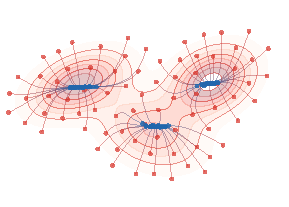
\includegraphics[width=.39\linewidth]{figures/generative-mean-shift-pde/trajectories.pdf}} &
\begin{tabular}{@{}cc@{}}
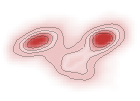
\includegraphics[width=.185\linewidth]{figures/generative-mean-shift-pde/snapshot-1.pdf} &
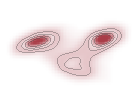
\includegraphics[width=.185\linewidth]{figures/generative-mean-shift-pde/snapshot-2.pdf} \\
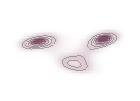
\includegraphics[width=.185\linewidth]{figures/generative-mean-shift-pde/snapshot-3.pdf} &
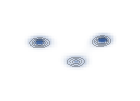
\includegraphics[width=.185\linewidth]{figures/generative-mean-shift-pde/snapshot-4.pdf}
\end{tabular}
\\[-.2em]
\small trajectories on the initial density & \small later density snapshots
\end{tabular}
\caption{\emph{Continuous-time mean shift for a densely sampled three-Gaussian mixture.} Left: initial density level sets, in red, and representative particle paths of $\dot x=M_\epsilon[\alpha_t](x)$, colored from red to blue. Right: four later kernel-density renderings of $\alpha_t$ at increasing times, with the same red-to-blue time palette; the initial density is omitted because it is shown on the left. The snapshots show the long multimodal transient before the globally positive Gaussian interactions drive the cloud toward the one-point consensus described in Remark~\ref{rem-mean-shift-consensus}.}
\label{fig:generative-mean-shift-pde}
\end{figure}
\index{kernel!Gaussian}% strictindex
\index{kernel!regression}% strictindex
\index{transport!PDE}% strictindex

\paragraph{Gradient structure and convergence.}
\index{gradient!structure}% strictindex

When the token space has dimension $d$ and the query/key space has dimension $r$, take $Q,K\in\RR^{r\times d}$ and $V\in\RR^{d\times d}$. If $V=Q^\top K$, the field $\Gamma_\theta[\alpha]$ is a gradient vector field in the token variable. Indeed, define the log-partition potential
\[
	\Phi_\alpha(x)
	=
	\int \exp(\dotp{Qx}{Ky})\d\alpha(y),
	\qquad
	U_\alpha(x)=\log\Phi_\alpha(x).
\]
Then
\[
	\nabla_x U_\alpha(x)
	=
	\frac{\int Q^\top K y\,\exp(\dotp{Qx}{Ky})\d\alpha(y)}
	     {\int \exp(\dotp{Qx}{Kz})\d\alpha(z)}
	=
	\Gamma_\theta[\alpha](x).
\]
This proves only that the velocity is an instantaneous gradient in $x$; it does not by itself identify a Wasserstein energy. Indeed, the natural scalar candidate $f_{\rm att}(\alpha)=\int U_\alpha(x)\,\d\alpha(x)$ has first variation
\[
	\delta f_{\rm att}(\alpha)(z)
	=
	U_\alpha(z)
	+
	\int
	\frac{\exp(\dotp{Qx}{Kz})}{\Phi_\alpha(x)}
	\,\d\alpha(x),
\]
up to an additive constant. The second term is the response of every query normalization to a perturbation of the key distribution, and its spatial gradient is absent from $\Gamma_\theta[\alpha]$. Thus, without additional symmetry or integrability conditions, the displayed attention PDE is a transportation dynamics rather than the Wasserstein gradient flow of this fixed scalar functional. Special variants recover additional structure: Sinkhorn attention can be interpreted through doubly stochastic normalization and Wasserstein-type gradient flows~\cite{Sander2022Sinkformers,Castin2025DynamicsTransformers}, while spherical normalization gives an idealized constrained token dynamics, not an exact model of practical layer normalization.
\index{transformer}% strictindex
\index{doubly stochastic normalization}% strictindex
\index{transport!equation}% strictindex
\index{controlled transport}% strictindex
\index{first variation}% strictindex
\index{layer normalization}% strictindex
\index{Wasserstein!gradient}% strictindex
\index{gradient!flow}% strictindex
\index{Wasserstein!gradient flow}% strictindex
\index{attention}% strictindex

Long-depth behavior depends on the weights and normalization. Fixed-weight Euclidean dynamics exhibit different cluster geometries after suitable rescaling~\cite{Geshkovski2023EmergenceClusters}. On the unit sphere, the projected model with $Q=K=\epsilon^{-1/2}\Id$, $V=\Id$ and $\epsilon>0$ reads
\begin{equation}\label{eq-spherical-attention-dynamics}
 \dot x_i=(\Id-x_ix_i^\top)
 \frac{\sum_j e^{\dotp{x_i}{x_j}/\epsilon}x_j}{\sum_j e^{\dotp{x_i}{x_j}/\epsilon}},
 \qquad x_i\in\mathbb S^{d-1}.
\end{equation}
For $d\geq2$, finitely many initial tokens lying in an open hemisphere converge exponentially to one common point~\cite[cone-collapse lemma]{Geshkovski2023MathematicalPerspective}. Two antipodal tokens can instead be stationary. At low temperature, separated clusters can persist for times exponentially large in $1/\epsilon$~\cite{GeshkovskiKoubbiPolyanskiyRigollet2024Metastability}; related mean-field clustering and geometric variants are studied in~\cite{Bruno2024MetastableClustering,Castin2025DynamicsTransformers}. Eventual consensus is therefore distinct from observable metastable clustering, and neither conclusion applies to arbitrary learned weights and architectures.

\paragraph{From token evolution to parameter training.}
A token law describes a forward computation; a law of head parameters describes optimization. Barboni et al.~\cite{BarboniDeHoopFuruyaPeyre2026TrainingTransformers} train an infinite-depth, many-head model with biased attention by a conditional Wasserstein flow. Their Theorem~4 gives local exponential convergence to zero risk under positive initial conditioning of the value-parameter part of the tangent kernel, an initial risk sufficiently small relative to that bound, and the stated regularity and moment hypotheses. This is neither an arbitrary-initialization result nor a theorem for the bias-free single-head model above.

Other analyses cover overparameterized shallow encoders~\cite{WuLiuChrysosCevher2023ShallowTransformers}, regularized deep mean-field models~\cite{Gao2024TrainingTransformers}, and coupled token/parameter limits with shallow regularized or deep local convergence results~\cite{HertyLiu2026MeanFieldTransformers}. Keeping training time distinct from depth links these models to the conditional ResNet geometry of Section~\ref{sec-conditional-wasserstein-resnets}, while preserving the distinction between the two evolving laws.

\section{Flows over the Gaussian Manifold}
\label{sec-gaussian-closure-transport-dynamics}
\index{Gaussian!manifold}% strictindex

Gaussian measures provide a useful testing ground for the preceding dynamics. They are not invariant under a general Wasserstein gradient flow: a nonlinear velocity usually creates non-Gaussian densities immediately. The useful substitute is to either identify affine velocities, which exactly preserve Gaussianity, or to project the dynamics onto the Gaussian manifold. In both cases the measure PDE reduces to matrix ODEs for the mean and covariance. This viewpoint is emphasized in the survey~\cite{Peyre2026OptimalDiffusionTransports} and is useful for comparing diffusion paths, Wasserstein gradient flows, drifting fields and transformer-type dynamics.
\index{affine!closure}% strictindex
\index{drifting!field}% strictindex
\index{Wasserstein!gradient}% strictindex
\index{gradient!flow}% strictindex
\index{transformer}% strictindex
\index{Wasserstein!gradient flow}% strictindex
\index{Gaussian!manifold}% strictindex
\index{Gaussian!measure}% strictindex

For constrained gradient flows on this family, the covariance equation is the finite-dimensional Bures--Wasserstein gradient flow on positive definite matrices. Thus Gaussian closure is not just a computational shortcut: it is the restriction of Wasserstein geometry to the Gaussian submanifold, where affine gradient fields encode tangent vectors. Figure~\ref{fig:gradflow-gaussian-closure} first compares three illustrative Gaussian paths from a source \(\alpha_0\) to a target \(\gamma\); the exact ambient equations admitting Gaussian solutions for specified energies \(f(\alpha)\) are catalogued afterwards in Proposition~\ref{prop-centered-gaussian-covariance-catalogue}.
\index{Gaussian!submanifold}% strictindex
\index{affine!gradient}% strictindex
\index{Bures!Wasserstein geometry}% strictindex
\index{Wasserstein!gradient}% strictindex
\index{Gaussian!closure}% strictindex
\index{gradient!flow}% strictindex

\begin{figure}[ht]
\centering
\begin{tabular}{@{}ccc@{}}
\small $\Wass_2$ geodesic & \small schematic covariance inflation & \small drifting closure \\[-.15em]
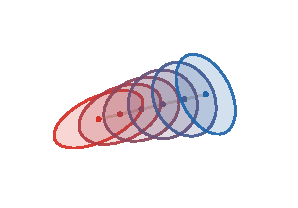
\includegraphics[width=.30\linewidth]{figures/gradflow-gaussian-closure/ot-ellipses.pdf} &
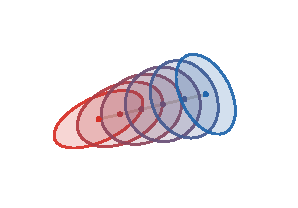
\includegraphics[width=.30\linewidth]{figures/gradflow-gaussian-closure/sinkhorn-ellipses.pdf} &
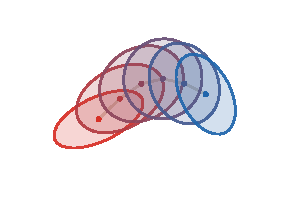
\includegraphics[width=.30\linewidth]{figures/gradflow-gaussian-closure/drifting-ellipses.pdf}
\end{tabular}
\caption{\emph{Three Gaussian paths from a red source $\alpha_0$ to a blue target $\gamma=\Gaussian(\bar m,\bar\Sigma)$.} The left panel is the constant-speed $\Wass_2$ geodesic, equivalently the displacement interpolation minimizing the Benamou--Brenier action between $\alpha_0$ and $\gamma$. The middle panel is only a schematic isotropic covariance inflation of that geodesic, obtained by adding a multiple of \(t(1-t)\Id\); it is not identified with a Sinkhorn geodesic or a Schr\"odinger bridge. The right panel is a prescribed non-variational drifting flow with an affine Gaussian-preserving velocity, chosen so that the mean follows a curved path while the covariance reaches the same endpoint $\gamma$.}
\index{moment matching}% strictindex
\index{Gaussian!closure}% strictindex
\index{velocity field}% strictindex
\label{fig:gradflow-gaussian-closure}
\end{figure}

\paragraph{Gaussianity preservation.}
\index{Gaussian!preservation}% strictindex

The first question is invariance: one wants a simple criterion ensuring that the continuity equation does not leave the finite-dimensional Gaussian family.
\index{continuity equation}% strictindex


\begin{prop}[Affine velocities preserve Gaussianity]\label{prop-gaussian-affine-closure}
\index{affine!closure}% strictindex
	Let $\alpha_0=\Gaussian(m_0,\Sigma_0)$, with $\Sigma_0\succ0$. Let $b_t\in\RR^d$ and $A_t\in\RR^{d\times d}$ be locally integrable on a time interval, and let $(m_t,\Sigma_t)$ solve
	\[
		\dot m_t=b_t,
		\qquad
		\dot\Sigma_t=A_t\Sigma_t+\Sigma_tA_t^\top,
		\qquad
		(m_{t=0},\Sigma_{t=0})=(m_0,\Sigma_0).
	\]
	Then, as long as this matrix ODE is defined, $\Sigma_t\succ0$ and
	\[
		\alpha_t=\Gaussian(m_t,\Sigma_t)
	\]
	is the solution of the continuity equation
	\[
		\partial_t\alpha_t+\diverg(\alpha_t v_t)=0,
		\qquad
		v_t(x)=b_t+A_t(x-m_t).
	\]
	In particular, if a smooth functional $f$ has a Wasserstein gradient on Gaussian measures of the affine form
	\[
		\Wgrad f(\Gaussian(m,\Sigma))(x)
		=
		b_f(m,\Sigma)+A_f(m,\Sigma)(x-m),
	\]
	with $A_f(m,\Sigma)$ symmetric, then the displayed moment ODE below produces a Gaussian distributional solution of the full Wasserstein gradient-flow equation for $f$:
	\[
		\dot m_t=h_f(m_t,\Sigma_t),
		\qquad
		\dot\Sigma_t=H_f(m_t,\Sigma_t),
	\]
	where
	\[
		h_f(m,\Sigma)=-b_f(m,\Sigma),
		\qquad
		H_f(m,\Sigma)
		=
		-\bigl(A_f(m,\Sigma)\Sigma+\Sigma A_f(m,\Sigma)\bigr).
	\]
	Conversely, fix a non-degenerate Gaussian \(\Gaussian(m,\Sigma)\). Suppose that a finite-energy Wasserstein tangent field \(V_{m,\Sigma}\) is represented by a gradient in \(L^2(\Gaussian(m,\Sigma))\) and is tangent to the Gaussian manifold at this Gaussian. Then there exist \(b(m,\Sigma)\) and a symmetric matrix \(A(m,\Sigma)\) such that
	\[
		V_{m,\Sigma}(x)=b(m,\Sigma)+A(m,\Sigma)(x-m)
		\qquad
		\Gaussian(m,\Sigma)\text{-a.e.}
	\]
	Consequently, under the same smoothness assumptions, if the Wasserstein gradient flow of a functional preserves the Gaussian family for all non-degenerate Gaussian initial data, then \(\Wgrad f(\Gaussian(m,\Sigma))\) is affine on each Gaussian. Without the Wasserstein gradient representative, this converse is false because one may add velocity fields with zero \(\Gaussian(m,\Sigma)\)-weighted divergence.
\index{affine!closure}% strictindex
\index{Wasserstein!gradient}% strictindex
\index{Gaussian!manifold}% strictindex
\index{divergence-free field}% strictindex

	Finally, any smooth Gaussian curve with positive definite covariance can be generated by an affine velocity. If one wants the velocity to be a Wasserstein tangent gradient, one chooses the unique symmetric solution of the Lyapunov equation
\index{affine!closure}% strictindex
\index{Lyapunov equation}% strictindex
	\[
		A_t\Sigma_t+\Sigma_t A_t=\dot\Sigma_t.
	\]
\end{prop}

\begin{proof}
	Let \(X_t\) follow the characteristic ODE \(\dot X_t=b_t+A_t(X_t-m_t)\) with \(X_0\sim\Gaussian(m_0,\Sigma_0)\). Since \(\dot m_t=b_t\), the centered variable \(\tilde X_t=X_t-m_t\) solves the homogeneous linear ODE \(\dot{\tilde X}_t=A_t\tilde X_t\). If \(\Phi_t\) is the fundamental matrix \(\dot\Phi_t=A_t\Phi_t\), \(\Phi_{t=0}=\Id\), then
	\[
		X_t=m_t+\Phi_t(X_0-m_0),
		\qquad
		\Sigma_t=\Phi_t\Sigma_0\Phi_t^\top.
	\]
	Hence \(X_t\) is Gaussian and \(\Sigma_t\succ0\), and
\index{random variable}% strictindex
	\[
		\dot\Sigma_t
		=
		\frac{\d}{\d t}\EE\bigl(\tilde X_t\tilde X_t^\top\bigr)
		=
		A_t\Sigma_t+\Sigma_t A_t^\top.
	\]
	This proves Gaussian preservation and the moment ODE\@. The Wasserstein gradient-flow statement follows by inserting the descent velocity $v_t=-\Wgrad f(\alpha_t)$.
\index{Wasserstein!gradient}% strictindex

	For the converse, fix $\alpha=\Gaussian(m,\Sigma)$ and denote its density by $\rho$. Tangency to the Gaussian manifold means that the density variation $-\diverg(\rho V)$ is generated by some moment variation $(\dot m,\dot\Sigma)$, with $\dot\Sigma$ symmetric. Set $b=\dot m$, and let $A=A^\top$ be the unique solution of
	\(A\Sigma+\Sigma A=\dot\Sigma\).
	By the first part of the proposition, the affine gradient field $V_0(x)=b+A(x-m)$ generates exactly the same infinitesimal Gaussian variation. Hence
	\(\diverg\bigl(\rho(V-V_0)\bigr)=0\)
	in the distributional sense. Both $V$ and $V_0$ belong to the $L^2(\alpha)$ closure of gradient fields. The weighted Helmholtz decomposition therefore makes $V-V_0$ simultaneously a tangent gradient and orthogonal to every tangent gradient, so $V=V_0$ in $L^2(\alpha)$. Equivalently, for a smooth representative $V-V_0=\nabla\psi$, integration by parts gives $\int\norm{\nabla\psi}^2\d\alpha=0$. This proves that the Wasserstein tangent representative is affine. The qualification is essential: without selecting the gradient representative, one can add a nonzero field with zero $\alpha$-weighted divergence without changing the Gaussian curve.
\index{Helmholtz decomposition}% strictindex

	For a prescribed smooth Gaussian curve, set $b_t=\dot m_t$ and choose any matrix $A_t$ satisfying $A_t\Sigma_t+\Sigma_tA_t^\top=\dot\Sigma_t$. Since $\Sigma_t$ is positive definite, the Lyapunov map $A\mapsto A\Sigma_t+\Sigma_t A$ is invertible on symmetric matrices, which gives the unique symmetric choice when a gradient velocity is required. In that case $v_t$ is the gradient of the quadratic potential $x\mapsto \dotp{b_t}{x}+\dotp{A_t(x-m_t)}{x-m_t}/2$.
\index{quadratic!potential}% strictindex
\index{gradient!velocity}% strictindex
\end{proof}

\paragraph{Gaussian-preserving gradient flows.}
\index{Gaussian!preservation}% strictindex
\index{gradient!flow}% strictindex

We now instantiate the affine-gradient viewpoint by tracking functionals whose full Wasserstein gradient is affine on Gaussian inputs. The catalogue below gives exact Gaussian solutions of the ambient Wasserstein equations, not projected or constrained flows. Whenever the ambient equation is unique in the solution class under consideration, this solution is the selected Wasserstein gradient flow and proves invariance of the Gaussian family; without such a uniqueness theorem, it still proves existence of a Gaussian distributional solution, but not invariance of every weak solution.
\index{Wasserstein!gradient}% strictindex
\index{moment functional}% strictindex

\begin{prop}[Gaussian closure catalogue]\label{prop-centered-gaussian-covariance-catalogue}
\index{Gaussian!covariance}% strictindex
\index{Gaussian!mean}% strictindex
\index{Gaussian!manifold}% strictindex
	Let \(\gamma=\Gaussian(\bar m,\bar\Sigma)\) on \(\RR^d\), with \(\bar\Sigma\succ0\), and let the initial condition be \(\alpha_0=\Gaussian(m_0,\Sigma_0)\), with \(\Sigma_0\succ0\). For each functional displayed below, evaluating its ambient Wasserstein gradient on a Gaussian gives an affine field. Consequently, as long as the following finite-dimensional ODE exists and \(\Sigma_t\succ0\),
	\[
		\alpha_t=\Gaussian(m_t,\Sigma_t)
	\]
	is an exact distributional solution of the corresponding ambient gradient-flow PDE, and its mean and covariance satisfy
	\[
		\dot{m}_t=h(m_t,\Sigma_t),
		\qquad
		\dot{\Sigma}_t=H(m_t,\Sigma_t).
	\]
	Write \(\delta_m=m-\bar m\), \(A=\bar\Sigma^{-1}\), and
	\[
		M_{\Sigma,\bar\Sigma}
		\eqdef
		\Sigma^{-1/2}\bigl(\Sigma^{1/2}\bar\Sigma\Sigma^{1/2}\bigr)^{1/2}\Sigma^{-1/2}.
	\]
	With the normalizations displayed in the first column, the mean vector field \(h\) and covariance vector field \(H\) are listed in the following table. If that PDE is unique in the selected solution class, this Gaussian solution is the Wasserstein flow from \(\alpha_0\). Gradients with respect to \(\Sigma\) are symmetric Frobenius gradients on the cone of covariance matrices.
	\index{maximum mean discrepancy}% strictindex
		\begin{center}
		\begingroup
		\small
		\renewcommand{\arraystretch}{1.55}
		\textbf{Exact Gaussian solutions of ambient Wasserstein gradient equations.}\par\smallskip
		\begin{tabularx}{\linewidth}{>{\raggedright\arraybackslash}p{.42\linewidth}>{\centering\arraybackslash}p{.18\linewidth}>{\raggedright\arraybackslash}X}
			\hline
			Functional \(f(\alpha)\) & \(h(m,\Sigma)\) & \(H(m,\Sigma)\) \\
			\hline
			\(g(m_\alpha,\Sigma_\alpha)\)
			&
			\(-\nabla_m g\)
			&
			\(-2(\Sigma\nabla_\Sigma g+\nabla_\Sigma g\,\Sigma)\)
			\\
			\(\displaystyle \int\Bigl(\frac12x^\top Bx+\dotp{\ell}{x}\Bigr)\d\alpha(x)\), \(B=B^\top\)
			&
			\(-(B m+\ell)\)
			&
			\(-(\Sigma B+B\Sigma)\)
			\\
			\(\displaystyle \frac14\iint (x-y)^\top G(x-y)\d\alpha(x)\d\alpha(y)\), \(G=G^\top\)
			&
			\(0\)
			&
			\(-(\Sigma G+G\Sigma)\)
			\\
			\(\KL(\alpha|\gamma)\)
			&
			\(-A\delta_m\)
			&
			\(2\Id-\Sigma A-A\Sigma\)
			\\
			\(\mathcal I(\alpha|\gamma)\)
			&
			\(-2A^2\delta_m\)
			&
			\(4\Sigma^{-1}-2\Sigma A^2-2A^2\Sigma\)
			\\
			\(\Wass_2^2(\alpha,\gamma)\)
			&
			\(-2\delta_m\)
			&
			\(2(M_{\Sigma,\bar\Sigma}\Sigma+\Sigma M_{\Sigma,\bar\Sigma}-2\Sigma)\)
			\\
			\(\MMD_k^2(\alpha,\gamma)\), \(k(x,y)=\dotp{x}{y}^2\)
			&
			\(-4R m\)
			&
			\(-4(\Sigma R+R\Sigma)\)
			\\
			\(\displaystyle \bar\MK_{\norm{\cdot-\cdot}^2}^{\epsilon}(\alpha,\gamma)\)
			&
			\(-2\delta_m\)
			&
			\(-2(\Sigma G_\epsilon+G_\epsilon\Sigma)\)
			\\
			\(\SW_2^2(\alpha,\gamma)\)
			&
			\(\displaystyle -\frac{2}{d}\delta_m\)
			&
			\(-2(\Sigma G_{\mathrm{sw}}+G_{\mathrm{sw}}\Sigma)\)
			\\
			\hline
		\end{tabularx}
		\endgroup
		\end{center}
		Here, in the MMD row,
	\[
		R=\Sigma+m\,m^\top-\bar\Sigma-\bar m\,\bar m^\top.
	\]
	The debiased Sinkhorn row uses the notation of Corollary~\ref{cor-gaussian-sinkhorn-divergence}: for Gaussian inputs,
	\[
		\bar\MK_{\norm{\cdot-\cdot}^2}^{\epsilon}(\alpha,\gamma)
		=
		\norm{\delta_m}^2+\Bb_\epsilon(\Sigma,\bar\Sigma)^2,
	\]
	with the closed-form covariance gradient
	\[
		G_\epsilon(\Sigma,\bar\Sigma)
		=
		\tau_\epsilon(\Sigma)
		-
		\bar\Sigma^{1/2}
		\tau_\epsilon\bigl(B_{\Sigma,\bar\Sigma}^{1/2}\bigr)
		B_{\Sigma,\bar\Sigma}^{-1/2}
		\bar\Sigma^{1/2},
		\qquad
		B_{\Sigma,\bar\Sigma}=\bar\Sigma^{1/2}\Sigma\bar\Sigma^{1/2}.
	\]
	Here \(\tau_\epsilon\) is the scalar function
	\[
		\tau_\epsilon(r)
		\eqdef
		\frac{\sqrt{\epsilon^2+16r^2}-\epsilon}{4r},
		\qquad r>0,
	\]
	applied to positive matrices by spectral calculus. Equivalently, for \(M\succ0\),
	\[
		\tau_\epsilon(M)
		=
		\bigl(\sqrt{\epsilon^2 \Id+16M^2}-\epsilon \Id\bigr)(4M)^{-1}.
	\]
	With this convention, \(G_\epsilon=\nabla_\Sigma \Bb_\epsilon(\Sigma,\bar\Sigma)^2\).
	In the sliced row, \(\sigma\) is the normalized spherical measure on \(\Sphere^{d-1}\), and
	\[
		G_{\mathrm{sw}}(\Sigma,\bar\Sigma)
		=
		\int_{\Sphere^{d-1}}
		\left(
			1-\sqrt{\frac{\theta^\top\bar\Sigma\theta}{\theta^\top\Sigma\theta}}
		\right)
		\theta\theta^\top\,\d\sigma(\theta).
	\]
	Here
	\[
		\mathcal I(\alpha|\gamma)
		=
		\int \left|\nabla\log\frac{\rho(x)}{\rho_\gamma(x)}\right|^2\rho(x)\,\d x
		=
		\int
		\left|\nabla\log\rho(x)+A(x-\bar m)\right|^2\rho(x)\,\d x
		\qquad(\alpha=\rho\,\d x),
	\]
	where $\rho_\gamma$ is the density of $\gamma$.
\end{prop}

\begin{proof}
	For the moment-functional row, the formula is exact on the full Wasserstein space. Indeed, write $m_\alpha=\int x\,\d\alpha(x)$ and $\Sigma_\alpha=\int (x-m_\alpha)(x-m_\alpha)^\top\d\alpha(x)$. If \(\eta\) is a signed perturbation with zero total mass, then $\d m_\alpha[\eta]=\int x\,\d\eta(x)$ and $\d\Sigma_\alpha[\eta]=\int (x-m_\alpha)(x-m_\alpha)^\top\d\eta(x)$. Thus, up to an irrelevant additive constant, the first variation is $\delta f(\alpha)(x)=\dotp{\nabla_m g}{x}+\dotp{\nabla_\Sigma g}{(x-m_\alpha)(x-m_\alpha)^\top}$,
	and its spatial gradient is the affine field
	\[
		\nabla_x\delta f(\alpha)(x)
		=
		\nabla_m g+2\nabla_\Sigma g\,(x-m_\alpha).
	\]
	Consequently the full Wasserstein descent velocity is affine, and Proposition~\ref{prop-gaussian-affine-closure} gives the displayed moment equations.
\index{moment functional}% strictindex
\index{first variation}% strictindex

	For the quadratic potential row, the ambient first variation is
	\[
		\delta f(\alpha)(x)=\frac12x^\top Bx+\dotp{\ell}{x},
		\qquad
		\nabla_x\delta f(\alpha)(x)=B m+\ell+B(x-m),
	\]
	which gives the displayed affine velocity. For the quadratic interaction row, the ambient first variation is $\delta f(\alpha)(x)=\frac12\int (x-y)^\top G(x-y)\d\alpha(y)$, with $\nabla_x\delta f(\alpha)(x)=G(x-m_\alpha)$.
	These first variations are quadratic in \(x\), hence the affine Gaussian flow coincides with the full Wasserstein gradient flow.
\index{quadratic!potential}% strictindex
\index{energy!interaction}% strictindex
\index{first variation}% strictindex

	For the KL row, write $\alpha=\rho\,\d x$ and let $\rho_\gamma$ denote the density of $\gamma$. The ambient first variation is \(\log(\rho/\rho_\gamma)\) up to an additive constant. If \(\alpha=\Gaussian(m,\Sigma)\), then
	\[
		\nabla\log(\rho/\rho_\gamma)(x)
		=
		-\Sigma^{-1}(x-m)+A(x-\bar m),
	\]
	so the descent velocity is
	\(v(x)=-A\delta_m+(\Sigma^{-1}-A)(x-m)\).
	Proposition~\ref{prop-gaussian-affine-closure} gives \(h(m,\Sigma)=-A\delta_m\) and \(H(m,\Sigma)=2\Id-\Sigma A-A\Sigma\). For the Fisher row, writing \(u=\log(\rho/\rho_\gamma)\), the ambient first variation of \(\frac12\mathcal I(\alpha|\gamma)\) is, up to constants,
	\[
		-\Delta u-\frac12|\nabla u|^2-\dotp{\nabla u}{\nabla\log\rho_\gamma}.
	\]
	For Gaussian \(\rho\) and Gaussian \(\gamma\), this is quadratic in \(x\). Multiplying by two for \(\mathcal I(\alpha|\gamma)\) gives the descent velocity
	\[
		v(x)=-2A^2\delta_m+2(\Sigma^{-2}-A^2)(x-m).
	\]
	Hence the Wasserstein velocity is affine and the Gaussian family is closed, with the displayed \(h\) and \(H\). Although the ambient Fisher flow is a fourth-order PDE for a generic density, it is therefore an exact finite-dimensional closure in this quadratic-reference case.
\index{Kullback-Leibler@Kullback--Leibler!divergence}% strictindex
\index{Fisher information}% strictindex

	For \(\Wass_2^2(\alpha,\gamma)\), the Brenier map from \(\Gaussian(m,\Sigma)\) to \(\gamma\) is
	\(T(x)=\bar m+M_{\Sigma,\bar\Sigma}(x-m)\).
	The descent velocity for the unhalved squared distance is \(2(T-\Id)\), which gives the mean and covariance equations through Proposition~\ref{prop-gaussian-affine-closure}. For the MMD row, \(k(x,y)=\dotp{x}{y}^2\) identifies the kernel mean embedding with the raw second moment. Thus
	\[
		\MMD_k^2(\alpha,\gamma)
		=
		\norm{\Sigma+m\,m^\top-\bar\Sigma-\bar m\,\bar m^\top}_{\mathrm F}^2
		=
		\norm{R}_{\mathrm F}^2,
	\]
	and the ambient first variation is \(2x^\top R x\), whose descent velocity is \(-4Rx\). This gives \(h(m,\Sigma)=-4R m\) and \(H(m,\Sigma)=-4(\Sigma R+R\Sigma)\).
\index{Brenier!map}% strictindex
\index{Bures!Wasserstein geometry}% strictindex
\index{maximum mean discrepancy}% strictindex
\index{second moment}% strictindex

	For the Sinkhorn row, Corollary~\ref{cor-gaussian-sinkhorn-divergence} gives the closed Gaussian formula as a squared mean displacement plus the smoothed Bures term \(\Bb_\epsilon^2\). This is not only a formula on the Gaussian submanifold. The first variation of the entropic value with respect to the first marginal is a Sinkhorn dual potential, and for Gaussian marginals the cross and self dual potentials are quadratic. Their debiased combination is therefore quadratic, so its spatial gradient is affine. This proves existence of the displayed Gaussian ambient solution; identifying it with every weak solution requires uniqueness in the chosen class. Since the restriction of the functional to Gaussians is
	\[
		(m,\Sigma)\mapsto \norm{m-\bar m}^2+\Bb_\epsilon(\Sigma,\bar\Sigma)^2,
	\]
	the quadratic coefficient is \(G_\epsilon=\nabla_\Sigma\Bb_\epsilon(\Sigma,\bar\Sigma)^2\), and the moment-functional computation gives the displayed \(h\) and \(H\). To compute this gradient, set \(B_{\Sigma,\bar\Sigma}=\bar\Sigma^{1/2}\Sigma\bar\Sigma^{1/2}\). Since \(\psi_\epsilon'(r)=-2\tau_\epsilon(r)\), differentiating
	\(\tr\psi_\epsilon(B_{\Sigma,\bar\Sigma}^{1/2})\) gives
	\[
		-\bar\Sigma^{1/2}
		\tau_\epsilon\bigl(B_{\Sigma,\bar\Sigma}^{1/2}\bigr)
		B_{\Sigma,\bar\Sigma}^{-1/2}
		\bar\Sigma^{1/2},
	\]
	whereas differentiating the self term
	\(-\frac12\tr\psi_\epsilon(\Sigma)\) gives \(\tau_\epsilon(\Sigma)\). This proves the displayed closed form for \(G_\epsilon\). When \(\bar\Sigma=\Id\), this covariance contribution is a spectral function of \(\Sigma\). If \(\lambda\) is an eigenvalue of \(\Sigma\), its covariance-eigenvalue derivative is
	\[
		4\sqrt{\lambda+\epsilon^2/16}-4\sqrt{\lambda^2+\epsilon^2/16},
	\]
			which is \(\dot\lambda\) in the displayed ODE. The centered spatial affine-velocity coefficient in that eigendirection is \(\dot\lambda/(2\lambda)\).

	For sliced Wasserstein, the exact ambient Wasserstein gradient is obtained by averaging the one-dimensional gradients. Each projection is Gaussian:
	\[
		(P_\theta)_\sharp\alpha=\Gaussian(\dotp{\theta}{m},\theta^\top\Sigma\theta),
		\qquad
		(P_\theta)_\sharp\gamma=\Gaussian(\dotp{\theta}{\bar m},\theta^\top\bar\Sigma\theta).
	\]
	Hence
	\[
		\SW_2^2(\alpha,\gamma)
		=
		\int_{\Sphere^{d-1}}
		\left[
			\dotp{\theta}{\delta_m}^2
			+
			\left(\sqrt{\theta^\top\Sigma\theta}
			-\sqrt{\theta^\top\bar\Sigma\theta}\right)^2
		\right]\d\sigma(\theta).
	\]
	If \(T_\theta\) is the monotone transport from \((P_\theta)_\sharp\alpha\) to \((P_\theta)_\sharp\gamma\), then the descent velocity for the unhalved sliced objective is
	\[
		2\int_{\Sphere^{d-1}}\bigl(T_\theta(P_\theta x)-P_\theta x\bigr)\theta\,\d\sigma(\theta).
	\]
	For Gaussian marginals, \(T_\theta\) is affine. Thus this velocity is affine in \(x\), and Proposition~\ref{prop-gaussian-affine-closure} applies. The spherical identity \(\int\theta\theta^\top\d\sigma(\theta)=\Id/d\) gives the mean equation, and differentiating the covariance term gives \(G_{\mathrm{sw}}\).
\index{Sinkhorn!divergence}% strictindex
\index{Gaussian!Sinkhorn}% strictindex
\index{sliced Wasserstein!distance}% strictindex
\index{one-dimensional!projection}% strictindex
\end{proof}

\begin{example}[Linear mean-field networks as cross-covariance flows]
\index{flow!cross-covariance}% strictindex
\index{cross-covariance}% strictindex
	Consider the two-layer mean-field model of Section~\ref{sec-wasserstein-flows-mlp}, and take the linear activation $\sigma(s)=s$, so that $\psi((u,v),z)=v\,\dotp{u}{z}$.
\index{two-layer neural network}% strictindex
	We restrict this example to centered neuron laws, $\int (u,v)\d\alpha(u,v)=0$, and write their covariance in blocks as
	\[
		\Sigma_\alpha=
		\begin{pmatrix}
			\Sigma_{u,u}(\alpha) & \Sigma_{u,v}(\alpha)\\
			\Sigma_{v,u}(\alpha) & \Sigma_{v,v}(\alpha)
		\end{pmatrix},
	\]
	and use the lower-left cross-covariance block
	\[
		\Sigma_{v,u}(\alpha)=\int v u^\top\d\alpha(u,v)\in\RR^{d'\times d}.
	\]
	The predictor is therefore the linear map $G_{\alpha_t}(z)=\Sigma_{v,u}(\alpha_t)z$. For the squared Euclidean loss, set $S=\int zz^\top\d\rho(z,y)$ and $R=\int y z^\top\d\rho(z,y)$.
\index{second moment}% strictindex
\index{neuron law}% strictindex
	The learning energy of~\eqref{eq-mlp-square-loss-quadratic-linear} is then the covariance functional
	\[
		f(\alpha)=g(\Sigma_\alpha),
		\qquad
		g(\Sigma)
		=
		\frac12\tr\!\big(\Sigma_{v,u}S\Sigma_{u,v}\big)
		-\tr\!\big(R\Sigma_{u,v}\big)
		+\frac12\int\norm{y}^2\d\rho(z,y).
	\]
	This puts the model exactly in the centered moment-functional row of Proposition~\ref{prop-centered-gaussian-covariance-catalogue}. To see that it recovers the usual particle equation, write $E_\alpha\eqdef \Sigma_{v,u}(\alpha)S-R$. The first variation is $\delta f(\alpha)(u,v)=\dotp{E_\alpha}{v u^\top}=v^\top E_\alpha u$.
\index{first variation}% strictindex
	Hence the particle velocity in parameter space is linear:
	\[
		-\nabla_{(u,v)}\delta f(\alpha)(u,v)
		=
		-\begin{pmatrix}
			0 & E_\alpha^\top \\
			E_\alpha & 0
		\end{pmatrix}
		\begin{pmatrix} u \\ v \end{pmatrix}.
	\]
	Equivalently, at the level of $g$, \(\nabla_\Sigma g=\frac12\begin{pmatrix}0 & E_\alpha^\top\\ E_\alpha & 0\end{pmatrix}\).
	The factor \(1/2\) in the covariance gradient comes from the symmetry of \(\Sigma\): the upper-right block is the transpose of the lower-left block. Substituting this gradient in Proposition~\ref{prop-centered-gaussian-covariance-catalogue} gives
	\[
		\dot m_t=0,
		\qquad
		\dot\Sigma_t=-(\Sigma_t L_t+L_t\Sigma_t),
		\qquad
		L_t=
		\begin{pmatrix}
			0 & E_t^\top\\
			E_t & 0
		\end{pmatrix},
		\qquad
		E_t=\Sigma_{v,u}(\alpha_t)S-R.
	\]
	Thus a centered Gaussian law of neurons remains centered Gaussian. The predictor and the residual $E_t$ depend only on the cross-covariance block, but this block does not generally evolve autonomously: the displayed matrix ODE couples it to $\Sigma_{u,u}$ and $\Sigma_{v,v}$. The closed state variable is the full covariance $\Sigma_t$. This exact Gaussian closure is special to the linear activation; for nonlinear activations, Gaussian closures are usually projections rather than invariant families.
\index{covariance!subblock}% strictindex
\index{neuron law}% strictindex
\index{neuron}% strictindex
\index{Gaussian!closure}% strictindex
\index{affine!closure}% strictindex
\end{example}

\paragraph{One-dimensional case.}
\index{Gaussian!one-dimensional}% strictindex
\index{Gaussian!closure}% strictindex

Fix a Gaussian target $\gamma=\Gaussian(\bar m,\bar\sigma^2)$, with $\bar\sigma>0$, and write $\alpha=\Gaussian(m,\sigma^2)$, with $\sigma>0$. By Proposition~\ref{prop-gaussian-w2-bures}, the parametrization $(m,\sigma)\mapsto\Gaussian(m,\sigma^2)$ identifies the one-dimensional Gaussian family with the open Euclidean half-plane. Hence every Gaussian-preserving functional in Proposition~\ref{prop-centered-gaussian-covariance-catalogue} is represented by the scalar restriction
\[
	g_f(m,\sigma)\eqdef f\bigl(\Gaussian(m,\sigma^2)\bigr).
\]
Set $\delta=m-\bar m$. For the Sinkhorn row below, with $\epsilon>0$, abbreviate
\[
	\psi_\epsilon(r)
	\eqdef
	-\frac{\sqrt{\epsilon^2+16r^2}-\epsilon}{2}
	-\frac{\epsilon}{2}
	\log\!\left(
		\frac{2\epsilon}{\sqrt{\epsilon^2+16r^2}+\epsilon}
	\right),
	\qquad r>0.
\]
The four restrictions used in Figure~\ref{fig:gradflow-gaussian-1d-energy-landscapes} are then
\begin{center}
\begingroup
\small
\renewcommand{\arraystretch}{1.55}
\begin{tabularx}{\linewidth}{>{\raggedright\arraybackslash}p{.34\linewidth}>{\raggedright\arraybackslash}X}
	\hline
	Functional $f(\alpha)$ & Scalar restriction $g_f(m,\sigma)$ \\
	\hline
	$\KL(\alpha\mid\gamma)$
	& $\displaystyle
	\log\frac{\bar\sigma}{\sigma}
	+\frac{\sigma^2+\delta^2}{2\bar\sigma^2}-\frac12$
	\\
	$\Wass_2^2(\alpha,\gamma)$
	& $\displaystyle \delta^2+(\sigma-\bar\sigma)^2$
	\\
	$\displaystyle \bar\MK_{\norm{\cdot-\cdot}^2}^{\epsilon}(\alpha,\gamma)$
	& $\displaystyle
	\delta^2+\psi_\epsilon(\sigma\bar\sigma)
	-\frac12\psi_\epsilon(\sigma^2)
	-\frac12\psi_\epsilon(\bar\sigma^2)$
	\\
	$\mathcal I(\alpha|\gamma)$
	& $\displaystyle
	\frac{\delta^2}{\bar\sigma^4}
	+\frac{(\sigma^2-\bar\sigma^2)^2}{\sigma^2\bar\sigma^4}$
	\\
	\hline
\end{tabularx}
\endgroup
\end{center}
The Sinkhorn formula is the one-dimensional specialization of Corollary~\ref{cor-gaussian-sinkhorn-divergence}; since $\psi_\epsilon(r)\to-2r$ as $\epsilon\downarrow0$, it recovers the squared-Wasserstein row. Figure~\ref{fig:gradflow-gaussian-1d-energy-landscapes} compares the four landscapes and their Euclidean gradient-flow trajectories. By Proposition~\ref{prop-centered-gaussian-covariance-catalogue}, these curves give exact Gaussian solutions of the ambient Wasserstein equations rather than the constrained Gaussian approximations introduced next; uniqueness of the ambient solution is a separate analytic issue.
\index{Kullback-Leibler@Kullback--Leibler!divergence}% strictindex
\index{Fisher information!relative}% strictindex
\index{Sinkhorn!divergence}% strictindex
\index{Wasserstein!Gaussian geometry}% strictindex

\begin{figure}[htbp]
\centering
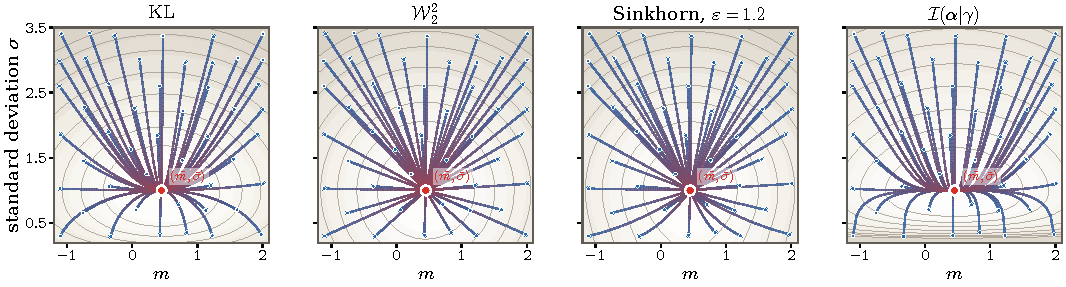
\includegraphics[width=\linewidth]{figures/gradflow-gaussian-1d-energy-landscapes/flows.pdf}
\caption{\emph{One-dimensional Gaussian Wasserstein gradient flows in the Euclidean parameter half-plane $(m,\sigma)$.} From left to right, the panels show relative entropy, squared Wasserstein distance, the debiased Sinkhorn divergence with $\epsilon=1.2$, and relative Fisher information. The same $48$ initial parameters are marked in blue; the trajectories progress through violet toward the common target $(\bar m,\bar\sigma)$ in red. Each background uses its own level scale to reveal the geometry of the corresponding energy. The $\Wass_2^2$ trajectories are straight rays, whereas the other functionals bend the evolution of the standard deviation.}
\label{fig:gradflow-gaussian-1d-energy-landscapes}
\end{figure}

\paragraph{Constrained evolution on the Gaussian manifold.}
\index{Gaussian!manifold}% strictindex

The preceding affine-gradient examples have a limited scope: most Wasserstein gradient flows of a functional \(f(\alpha)\) are not closed on the Gaussian manifold. A nonlinear ambient velocity creates higher-order moments immediately, so the exact Gaussian closure usually fails. The constrained viewpoint deliberately replaces the full evolution by its projection onto \(\mathcal G\), forcing the curve to remain Gaussian while keeping the Wasserstein tangent geometry.
\index{affine!closure}% strictindex
\index{Gaussian!projection}% strictindex

Let
\[
	\mathcal G=\{\Gaussian(m,\Sigma):m\in\RR^d,\ \Sigma\succ0\}
\]
be the Gaussian submanifold of $\Pp_2(\RR^d)$. The Wasserstein gradient of a functional constrained to a smooth submanifold $\mathcal M\subset\Pp_2$ is defined as the Riesz representative of the differential restricted to tangent velocities of $\mathcal M$. Its descent flow is formally the small-step limit of the constrained JKO scheme, whenever these minimizers exist and converge to a smooth curve:
\index{Gaussian!submanifold}% strictindex
\index{Wasserstein!gradient}% strictindex
\index{JKO scheme}% strictindex
\[
	\alpha^{(\ell+1)}\in
	\uargmin{\alpha\in\mathcal M}
	\frac{1}{2\tau}\Wass_2^2(\alpha,\alpha^{(\ell)})+f(\alpha).
\]
For $\mathcal M=\mathcal G$, tangent velocities are affine gradient fields $v(x)=b+A(x-m)$ with $A=A^\top$. The constrained gradient is therefore the $L^2(\Gaussian(m,\Sigma))$ projection of the ambient Wasserstein gradient onto this finite-dimensional affine space, whenever the ambient gradient exists.
\index{affine!gradient}% strictindex
\index{Wasserstein!gradient}% strictindex

\begin{prop}[Gaussian-constrained Wasserstein gradients]\label{prop-gaussian-gradient-bullet-list}
	Let $f$ be a smooth functional and assume that its restriction to nondegenerate Gaussian measures can be written as
\index{Gaussian!measure}% strictindex
	\[
		f(\Gaussian(m,\Sigma))=F(m,\Sigma).
	\]
	Then the Wasserstein gradient constrained to the Gaussian family is the affine vector field
\index{Wasserstein!gradient}% strictindex
	\[
		v_F(x)
		=
		\nabla_m F(m,\Sigma)
		+
		2\nabla_\Sigma F(m,\Sigma)(x-m),
	\]
	where $\nabla_\Sigma F$ denotes the symmetric matrix derivative. Equivalently, $v_F$ is the $L^2(\Gaussian(m,\Sigma))$ projection of the ambient Wasserstein gradient onto affine gradient fields, whenever the ambient gradient exists. Hence the gradient descent flow constrained to Gaussian measures satisfies
\index{affine!gradient}% strictindex
\index{Wasserstein!gradient}% strictindex
\index{Gaussian!measure}% strictindex
	\begin{equation}\label{eq-gaussian-wgf-closure}
		\dot m_t=-\nabla_m F(m_t,\Sigma_t),
		\qquad
		\dot\Sigma_t=-2\bigl(\Sigma_t\nabla_\Sigma F(m_t,\Sigma_t)+\nabla_\Sigma F(m_t,\Sigma_t)\Sigma_t\bigr),
	\end{equation}
	and the descent velocity is affine.
\end{prop}

\begin{proof}
	Test the functional along a Gaussian tangent vector, represented by an affine gradient field
\index{affine!gradient}% strictindex
	\(v(x)=b+A(x-m)\)
	with $A$ symmetric. The induced first-order variations are $\dot m=b$ and $\dot\Sigma=A\Sigma+\Sigma A$. Therefore
	\[
		\d F(m,\Sigma)[b,A\Sigma+\Sigma A]
		=
		\dotp{\nabla_m F}{b}
		+
		\tr\!\left(\nabla_\Sigma F(A\Sigma+\Sigma A)\right).
	\]
	Since $A$, $\Sigma$ and $\nabla_\Sigma F$ are symmetric, the second term equals
	\[
		2\,\tr(\nabla_\Sigma F\,A\Sigma)
		=
		\int \dotp{2\nabla_\Sigma F(x-m)}{A(x-m)}\d\Gaussian(m,\Sigma)(x).
	\]
	Together with the mean term, this gives
	\[
		\d F(m,\Sigma)[\dot m,\dot\Sigma]
		=
		\int \dotp{v_F(x)}{v(x)}\d\Gaussian(m,\Sigma)(x)
	\]
	for all affine gradient fields $v$. This identifies the constrained Wasserstein gradient in the induced $L^2(\alpha)$ metric, or equivalently the projection of the ambient gradient when it exists. Substituting the descent velocity $-v_F$ in Proposition~\ref{prop-gaussian-affine-closure} gives~\eqref{eq-gaussian-wgf-closure}.
\index{Wasserstein!gradient}% strictindex
\index{affine!closure}% strictindex
\end{proof}

This proposition is the organizing rule for constrained Gaussian closures: once the scalar energy has been reduced to a function of $(m,\Sigma)$, its constrained Wasserstein gradient is automatically affine and the covariance follows the Bures-type ODE~\eqref{eq-gaussian-wgf-closure}. When the first variation of $f$ is quadratic, this constrained gradient coincides with the full Wasserstein gradient.
\index{first variation}% strictindex
\index{Gaussian!closure}% strictindex


\paragraph{Non-variational Gaussian-preserving flows.}
\index{Gaussian!preservation}% strictindex
\index{Gaussian!preserving flow}% strictindex

The last examples are not ordinary gradient flows of a fixed scalar energy on the full Wasserstein space. They preserve Gaussianity because the prescribed velocity field is affine when evaluated on Gaussian measures.
\index{velocity field}% strictindex
\index{Wasserstein!space}% strictindex
\index{Gaussian!measure}% strictindex
\index{gradient!flow}% strictindex

\begin{example}[Flow matching and diffusion paths between Gaussians]
	Consider a prescribed Gaussian interpolation $\alpha_t=\Gaussian(m_t,\Sigma_t)$. Proposition~\ref{prop-gaussian-affine-closure} shows that an exact flow-matching velocity can be taken affine:
\index{affine!closure}% strictindex
\index{flow matching}% strictindex
	\[
		v_t(x)=\dot m_t+A_t(x-m_t),
		\qquad
		A_t\Sigma_t+\Sigma_t A_t=\dot\Sigma_t.
	\]
	In the isotropic case $\Sigma_t=s_t^2\Id$, this reduces to the transparent formula $v_t(x)=\dot m_t+\frac{\dot s_t}{s_t}(x-m_t)$. For instance, the diffusion noising path $X_t=a_tX_0+\sigma_t Z$, where $Z\sim\Gaussian(0,\Id)$ is independent of $X_0$,
	has $m_t=a_tm_0$ and $\Sigma_t=a_t^2\Sigma_0+\sigma_t^2\Id$. Thus, in the Gaussian case, diffusion paths and flow-matching paths reduce to the same mean-covariance bookkeeping, although the corresponding training objectives are different.
\index{flow matching}% strictindex
\end{example}

\begin{example}[Gaussian kernel drifting]
\index{kernel!Gaussian}% strictindex
\index{Gaussian!kernel drifting}% strictindex
	Let the target be $\gamma=\Gaussian(\bar m,\bar\Sigma)$ and assume $\al_t=\Gaussian(m_t,\Sigma_t)$. For the Gaussian kernel
	\[
		K_\epsilon(x,y)=\exp(-\norm{x-y}^2/(2\epsilon)),
	\]
	the normalized field~\eqref{eq-normalized-kernel-drift} satisfies
	\[
		B_\epsilon[\al_t](x)
		=
		-\epsilon(\Sigma_t+\epsilon\Id)^{-1}(x-m_t).
	\]
	Indeed the smoothed density \(x\mapsto\int K_\epsilon(x,y)\d\al_t(y)\) is proportional to the Gaussian density with mean $m_t$ and covariance $\Sigma_t+\epsilon\Id$. Thus \(B_\epsilon[\al_t]\) is the mean-shift vector of a Gaussian density: it points linearly toward the Gaussian mode, with strength set by the bandwidth. The drifting velocity~\eqref{eq-cross-minus-self-drift} is therefore the difference of two affine mean-shift fields; it is affine and preserves Gaussianity. With $A_t=(\Sigma_t+\epsilon\Id)^{-1}$ and $\bar A=(\bar\Sigma+\epsilon\Id)^{-1}$, the ODE is
	\[
		\dot m_t=\epsilon\bar A(\bar m-m_t),
		\qquad
		\dot\Sigma_t=\epsilon\bigl((A_t-\bar A)\Sigma_t+\Sigma_t(A_t-\bar A)\bigr).
	\]
	This finite-dimensional model explains the stabilizing role of the self-normalized repulsion term in drifting: without it, the covariance equation loses the $A_t\Sigma_t+\Sigma_tA_t$ contribution.
\end{example}

\begin{example}[Gaussian closure of attention dynamics]
\index{Gaussian!closure}% strictindex
\index{attention}% strictindex
	For the transformer PDE~\eqref{eq-transformer-mean-field-pde}, assume $\alpha=\Gaussian(m,\Sigma)$. Exponential tilting gives directly
\index{transformer}% strictindex
	$\Gamma_\theta[\alpha](x)=Vm+V\Sigma K^\top Qx$, which is affine. The Gaussian token law is preserved and satisfies
	\[
		\dot m_t=(V_t+V_t\Sigma_tK_t^\top Q_t)m_t,
		\qquad
		\dot\Sigma_t=B_t\Sigma_t+\Sigma_tB_t^\top,
		\qquad
		B_t=V_t\Sigma_tK_t^\top Q_t.
	\]
	When $V_t=Q_t^\top K_t$, the matrix $B_t=Q_t^\top K_t\Sigma_tK_t^\top Q_t$ is symmetric positive semidefinite, matching the gradient-field case mentioned above.
	This closure is not a convergence theorem for trained transformers. It is instead a tractable model of how attention can shear, amplify or contract a cloud of tokens through its covariance.
\index{transformer}% strictindex
\index{attention}% strictindex
\end{example}

\paragraph{Contractive Gaussian projection.}
\index{Gaussian!projection}% strictindex
\index{contractive Gaussian projection}% strictindex

The preceding examples show when Gaussianity is preserved or imposed by projection. Gelbrich's inequality~\cite{gelbrich1990formula} gives a useful variational explanation: replacing a measure by the Gaussian with the same first two moments cannot increase its Wasserstein distance to another similarly projected measure.
\index{Gelbrich inequality}% strictindex
\index{Wasserstein!distance}% strictindex

\begin{defn}[Gaussian projection]\label{def-gaussian-projection}
For \(\alpha\in\Pp_2(\RR^d)\), its Gaussian projection is
\[
	\GaussProj(\alpha)
	\eqdef
	\Gaussian(m_\alpha,\Sigma_\alpha),
\]
the Gaussian with the same mean and covariance as \(\alpha\).
\end{defn}

\begin{thm}[Gelbrich theorem]\label{thm-gelbrich-projection}
\index{Gelbrich theorem}% strictindex
	For every $\al,\be\in\Pp_2(\RR^d)$,
	\[
		\Wass_2^2\bigl(\GaussProj(\al),\GaussProj(\be)\bigr)
		=
		\norm{m_\al-m_\be}^2+\Bb^2(\Sigma_\al,\Sigma_\be)
		\leq
		\Wass_2^2(\al,\be).
	\]
\end{thm}

\begin{proof}
	Take any coupling $(X,Y)$ of $\al$ and $\be$, center the variables, and write $C=\EE[(X-m_\al)(Y-m_\be)^\top]$. In the positive definite case, positivity of the block covariance matrix implies the factorization $C=\Sigma_\al^{1/2}K\Sigma_\be^{1/2}$ with $\norm{K}_{\mathrm{op}}\leq1$, and therefore, by operator/nuclear norm duality, $\tr C\leq \tr\bigl((\Sigma_\al^{1/2}\Sigma_\be\Sigma_\al^{1/2})^{1/2}\bigr)$.
\index{covariance!matrix}% strictindex
	The semidefinite case follows by adding $\eta\Id$ to both covariance matrices and letting $\eta\downarrow0$.
	Expanding $\EE\norm{X-Y}^2$ gives the lower bound
	\[
		\EE\norm{X-Y}^2
		\geq
		\norm{m_\al-m_\be}^2+\Bb^2(\Sigma_\al,\Sigma_\be).
	\]
	Taking the infimum over couplings proves the inequality, while equality for Gaussian laws is Proposition~\ref{prop-gaussian-w2-bures}.
\end{proof}

Proposition~\ref{prop-gaussian-barycenter} is an earlier application of this contraction: because every Gaussian input is fixed by $\GaussProj$, projecting any competitor cannot increase the quadratic Wasserstein barycenter objective.

The following preservation criterion is a direct consequence of Gelbrich's theorem and was explained to us by Hugo Lavenant. It says that a functional which does not increase under moment-matched Gaussian projection admits Gaussian minimizing movements from Gaussian initial data.
\index{Gelbrich inequality}% strictindex
\index{moment matching}% strictindex
\index{Lavenant criterion}% strictindex
\index{Gaussian!projection}% strictindex
\index{minimizing movement}% strictindex
\index{Gelbrich theorem}% strictindex

\begin{thm}[Hugo Lavenant Gaussian-preservation criterion]\label{thm-lavenant-gaussian-preserving-jko}
\index{Gaussian!preservation}% strictindex
	Let $f:\Pp_2(\RR^d)\to(-\infty,+\infty]$ satisfy
	\[
		f\bigl(\GaussProj(\al)\bigr)\leq f(\al)
		\qquad\forall\al\in\Pp_2(\RR^d),
	\]
	with $\GaussProj$ defined in Definition~\ref{def-gaussian-projection}. If $\gamma$ is Gaussian and $\alpha^\star$ minimizes the JKO step
\index{Gelbrich inequality}% strictindex
	\[
		\eta\mapsto f(\eta)+\frac1{2\tau}\Wass_2^2(\gamma,\eta),
	\]
	then $\GaussProj(\alpha^\star)$ is also a minimizer. If this JKO minimizer is unique, it is Gaussian. Consequently, if every step from Gaussian data has a unique minimizer and the resulting minimizing movements converge in $\Wass_2$, each discrete iterate is Gaussian and every limit curve is Gaussian as well, possibly with a singular limiting covariance.
\index{Wasserstein!gradient}% strictindex
\index{gradient!flow}% strictindex
\index{Wasserstein!gradient flow}% strictindex
\index{JKO scheme}% strictindex
\end{thm}

\begin{proof}
	For the JKO claim, $\GaussProj(\gamma)=\gamma$ because $\gamma$ is Gaussian. Hence, for any competitor $\eta$,
	\[
		f\bigl(\GaussProj(\eta)\bigr)+\frac1{2\tau}\Wass_2^2\bigl(\gamma,\GaussProj(\eta)\bigr)
		\leq
		f(\eta)+\frac1{2\tau}\Wass_2^2(\gamma,\eta).
	\]
	Applying this to a minimizer $\eta=\alpha^\star$ shows that $\GaussProj(\alpha^\star)$ is again a minimizer. Uniqueness forces $\alpha^\star=\GaussProj(\alpha^\star)$.
\end{proof}

\paragraph{Moment closure beyond Gaussianity.}
\index{moment closure}% strictindex
\index{eikonal equation}% strictindex

Gaussian preservation concerns the full law, whereas moment closure asks only whether selected statistics obey an autonomous system. The first row of Proposition~\ref{prop-centered-gaussian-covariance-catalogue} in fact gives a distribution-free closure. If $f(\alpha)=g(m_\alpha,\Sigma_\alpha)$ and $G=\nabla_\Sigma g(m_\alpha,\Sigma_\alpha)$ denotes the symmetric Frobenius gradient, then the Wasserstein descent velocity is
\(v_\alpha(x)=-\nabla_m g(m_\alpha,\Sigma_\alpha)-2G(x-m_\alpha)\).
It is affine in $x$ for every $\alpha$, not only for Gaussian laws. Consequently, every sufficiently regular flow starting from an arbitrary $\alpha_0\in\Pp_2(\RR^d)$ satisfies
\begin{equation}\label{eq-distribution-free-mean-covariance-closure}
	\dot m_t=-\nabla_m g(m_t,\Sigma_t),
	\qquad
	\dot\Sigma_t
	=
	-2\bigl(\Sigma_t\nabla_\Sigma g(m_t,\Sigma_t)
	+\nabla_\Sigma g(m_t,\Sigma_t)\Sigma_t\bigr).
\end{equation}
For Gaussian initial data, this affine velocity also preserves Gaussianity; for general initial data, the law need not become Gaussian, but its mean and covariance still follow the same closed vector field $(h,H)$ listed in that proposition.

This suggests asking which linear statistics $\alpha\mapsto\int\varphi\,\d\alpha$ admit an exact closure. For scalar statistics, the answer is completely characterized by an eikonal equation.

\begin{prop}[Scalar moment closure and eikonal characterization]\label{prop-scalar-moment-closure}
	Let $\Omega\subset\RR^d$ be connected and open, let $\varphi\in C^2(\Omega)$, and set
	\(m_\varphi(\alpha)\eqdef\int_\Omega\varphi(x)\d\alpha(x)\)
	for probability measures such that $\varphi$ and $\norm{\nabla\varphi}^2$ are integrable. For every smooth $g:\RR\to\RR$, the Wasserstein gradient flow of $f_g(\alpha)=g(m_\varphi(\alpha))$ satisfies, whenever the differentiation is justified,
	\[
		\dot m_t
		=
		-g'(m_t)\int_\Omega\norm{\nabla\varphi(x)}^2\d\alpha_t(x),
		\qquad m_t=m_\varphi(\alpha_t).
	\]
	This equation is autonomous for every $g$, meaning that its right-hand side depends on $\alpha_t$ only through $m_t$, if and only if there are constants $a,b\in\RR$ such that
	\begin{equation}\label{eq-scalar-moment-affine-carre}
		\norm{\nabla\varphi(x)}^2=a+b\varphi(x)
		\qquad (x\in\Omega).
	\end{equation}
	In that case, $\dot m_t=-(a+b m_t)g'(m_t)$.
	Moreover, on every connected open set $U\subset\{x:\nabla\varphi(x)\neq0\}$, the restriction of~\eqref{eq-scalar-moment-affine-carre} to $U$ is equivalent to the existence of an eikonal coordinate $r\in C^2(U)$ and constants $c,\kappa,\lambda\in\RR$ such that
	\begin{equation}\label{eq-scalar-moment-eikonal-form}
		\norm{\nabla r}=1,
		\qquad
		\varphi=c+\kappa r+\frac{\lambda}{2}r^2.
	\end{equation}
	Under~\eqref{eq-scalar-moment-affine-carre}, one may take $\lambda=b/2$.
\end{prop}

\begin{proof}
	The first variation is $\delta f_g(\alpha)(x)=g'(m_\varphi(\alpha))\varphi(x)$, so the continuity equation gives the displayed evolution of $m_t$. Condition~\eqref{eq-scalar-moment-affine-carre} then proves sufficiency.

	For necessity, it is enough to take $g(s)=s$ and write $\psi=\norm{\nabla\varphi}^2$. Autonomy for Dirac laws first shows that $\psi=q\circ\varphi$ for some function $q$ on $\varphi(\Omega)$. Because $\Omega$ is connected, $\varphi(\Omega)$ is an interval. Comparing a Dirac law with any two-point mixture having the same $\varphi$-moment shows that
	\[
		q\bigl((1-\zeta)s_0+\zeta s_1\bigr)
		=
		(1-\zeta)q(s_0)+\zeta q(s_1)
		\qquad (0\leq\zeta\leq1).
	\]
	Hence $q$ is affine, which is precisely~\eqref{eq-scalar-moment-affine-carre}.

	On a regular set $U$, the right-hand side of~\eqref{eq-scalar-moment-affine-carre} is positive. Fix $s_0\in\varphi(U)$ and define $r(x)=\int_{s_0}^{\varphi(x)}(a+bs)^{-1/2}\d s$.
	Then $\norm{\nabla r}=1$. Inverting this change of variables gives~\eqref{eq-scalar-moment-eikonal-form} with $c=s_0$, $\kappa=\sqrt{a+bs_0}$, and $\lambda=b/2$. Conversely,~\eqref{eq-scalar-moment-eikonal-form} gives
	$\norm{\nabla\varphi}^2=\kappa^2-2\lambda c+2\lambda\varphi$.
\end{proof}

\begin{example}[A closed signed-distance moment]
	Let $\mathcal S$ be a $C^2$ hypersurface and let $r_{\mathcal S}$ be its signed distance on a sufficiently small tubular neighborhood $U$, where $\norm{\nabla r_{\mathcal S}}=1$. For
	$\varphi(x)=r_{\mathcal S}(x)+\lambda r_{\mathcal S}(x)^2/2$, one has $\norm{\nabla\varphi}^2=1+2\lambda\varphi$. Consequently, for any solution whose support remains in $U$, the scalar moment obeys $\dot m_t=-(1+2\lambda m_t)g'(m_t)$ under the objective $f_g(\alpha)=g(\int\varphi\,\d\alpha)$.
	For $\lambda=0$ and a genuinely curved $\mathcal S$, the observable is generally non-polynomial and the descent velocity is proportional to the non-affine normal field $\nabla r_{\mathcal S}$. This closure therefore does not arise from the mean--covariance mechanism above.
\end{example}
